\documentclass[12pt]{ucthesis}

% ------------------- Import packages ---------------------------
\usepackage{etex}
\usepackage[morefloats=125]{morefloats}
\usepackage[hyphens]{url}
\usepackage{subfig}
\usepackage{graphicx}
\usepackage{tabularx}
\usepackage{amssymb}
\usepackage{amsmath}
\usepackage[letterpaper]{geometry}
\usepackage[overload]{textcase}
\usepackage{color}
\usepackage{soul}
\usepackage[nonumberlist,toc]{glossaries}
\usepackage{wrapfig}
\usepackage{longtable}
\usepackage{morefloats}
\usepackage{float}
\usepackage{listings}
\usepackage{makecell}
\usepackage{appendix}
\usepackage[]{algorithm2e}
\usepackage{titlesec}
\usepackage[breaklinks=true,hidelinks,pdfusetitle]{hyperref}
\usepackage{cleveref}
\usepackage{ifthen}
\usepackage{bm}
\usepackage[table,xcdraw]{xcolor}
\usepackage{placeins}
\usepackage[tableposition=top]{caption}
\usepackage[framed,numbered,autolinebreaks,useliterate]{mcode}


% ------------- Define new commands -------------------------
\newcommand{\keyword}[1]{\textbf{#1}}
\newcommand{\tabhead}[1]{\textbf{#1}}
\newcommand{\code}[1]{\texttt{#1}}
\newcommand{\mat}[1]{\mathbf{#1}}
\newcommand{\file}[1]{\texttt{\bfseries#1}}
\newcommand{\option}[1]{\texttt{\itshape#1}}
\newcommand{\decoRule}{\rule{.8\textwidth}{.4pt}} % New command for a rule to be used under figures
\newcommand{\units}[1]{\ \left[\mathsf{#1} \right]} % create a units command
\newcommand{\vech}[1]{\mathbf{\hat{#1}}} % create unit vector with a hat
\newcommand{\norm}[1]{\left\Vert #1 \right\Vert} % create vector norm notation
\newcommand{\todo}[1]{\hl{\textbf{TODO: #1}}} % create todo flag

\setcounter{secnumdepth}{3}
\setcounter{tocdepth}{3}

\makeindex
\makeglossaries

% Shrink the size of headers
\titleformat{\chapter}[display]
        {\normalfont\normalsize\centering}
        {\ifthenelse{\equal{\thechapter}{A}}{APPENDICES\\[4.3ex]}{}\chaptertitlename\ \thechapter}
        {0pt}{\normalsize\uppercase}
\titlespacing*{\chapter}{0pt}{-20pt}{4.3ex plus .2ex}


\titleformat*{\section}{\normalsize\bfseries}
\titleformat*{\subsection}{\small\bfseries}
\titleformat*{\subsubsection}{\small\bfseries}
\titleformat*{\paragraph}{\small\bfseries}
\titleformat*{\subparagraph}{\small\bfseries}

\bibliographystyle{abbrv}

% Make \tindent indent pages if you have no paragraph indent
\newlength\tindent
\setlength{\tindent}{\parindent}
\setlength{\parindent}{0.in} \setlength{\parskip}{1.em}
\renewcommand{\indent}{\hspace*{\tindent}}
% Otherwise, comment out the above and uncomment this for default indentation on each paragraph
%\setlength{\parindent}{0.25in} \setlength{\parskip}{6pt}

\geometry{verbose,nohead,tmargin=1in,bmargin=1in,lmargin=1.5in,rmargin=1in}

% Different font in captions (single-spaced, bold) ------------
\newcommand{\captionfonts}{\small\bf\ssp}

\newcommand{\mycaption}[2]{\caption[#1 --- #2]{#1 --- #2}}

\makeatletter  % Allow the use of @ in command names
\long\def\@makecaption#1#2{%
  \vskip\abovecaptionskip
  \sbox\@tempboxa{{\captionfonts #1: #2}}%
  \ifdim \wd\@tempboxa >\hsize
    {\captionfonts #1: #2\par}
  \else
    \hbox to\hsize{\hfil\box\@tempboxa\hfil}%
  \fi
  \vskip\belowcaptionskip}
\makeatother   % Cancel the effect of \makeatletter
% ---------------------------------------

% Define Appendix refs
\crefname{app}{appendix}{appendices}
\Crefname{app}{Appendix}{Appendices}

% Add Figures folder to the graphics path
\graphicspath{{Figures/}{figures/}}

% Options for hyperref
\hypersetup{
    bookmarksnumbered=true,
    bookmarksopen=false,
    bookmarksopenlevel=0,
    colorlinks=false,
    pdfstartview=Fit,
    pdfborder={0 0 0},
}

\newcounter{qcounter}
\providecommand{\keywords}[1]{\textbf{\textit{Keywords:}} #1}


\begin{document}

% Declarations for Front Matter
\title{Development of a Model and Imbalance Detection System for the Cal Poly Wind Turbine}
\author{Ryan Takatsuka}
\degreemonth{June} \degreeyear{2019} \degree{Master of Science}
\defensemonth{May} \defenseyear{2019}
\numberofmembers{2}
   \chair{John Ridgely, Ph.D. \linebreak Professor of Mechanical Engineering}
   \othermemberA{Glen Thorncroft, Ph.D. \linebreak Professor of Mechanical Engineering}
   \othermemberB{Patrick Lemieux, Ph.D. \linebreak Professor of Mechanical Engineering}
\field{Mechanical Engineering} \campus{San Luis Obispo}
\copyrightyears{seven}


\maketitle

\begin{frontmatter}

% Custom made for Cal Poly (by Mark Barry, modified by Andrew Tsui).
\copyrightpage

% Custom made for Cal Poly (by Andrew Tsui).
\committeemembershippage

\begin{abstract}
This thesis develops a model of the Cal Poly Wind Turbine that is used to determine if there is an imbalance in the turbine.  A theoretical model is derived to estimate the expected vibrations when there is an imbalance in the rotor.  Vibration and acceleration data are collected from the turbine tower during operation to confirm the model is useful and accurate for determining imbalances in the turbine.  

Various signal processing techniques for analyzing the vibration data are explored and tested with the simulation.  This includes frequency shifts, lock-in amplifiers, phase-locked loops, discrete Fourier transforms, and various filters.  The processed data is fed into an algorithm that determines if there is an imbalance.

The detection algorithm consists of a machine learning classification model that uses experimental data to train and increase the success rate of the imbalance detection.  The model uses the maximum frequency component and magnitude as an input to classify the data as ``balanced" or ``not balanced" using the K-nearest neighbors algorithm.  While this classification algorithm requires slightly more computational power than others, it is simple to implement and has a high accuracy rating.

\todo{Add a quick summary of the results.}


\end{abstract}

%\begin{acknowledgements}
%\noindent
Thanks to:
\begin{itemize}
    \item Andrew Guenther, for uploading this template
\end{itemize}

%\end{acknowledgements}

\tableofcontents

\listoftables

\listoffigures

% Add CHAPTER into table of contents.
\addtocontents{toc}{%
   \noindent CHAPTER
}

\end{frontmatter}

\pagestyle{plain}

\renewcommand{\baselinestretch}{1.66}

\chapter{Introduction} % Main chapter title

\label{ch_introduction} % Change X to a consecutive number; for referencing this chapter elsewhere, use \ref{Chapter1}

%----------------------------------------------------------------------------------------
%	SECTION 1
%----------------------------------------------------------------------------------------
\section{System Overview}

The wind turbine that is analyzed in this thesis is part of the Cal Poly Wind Power Research Center.  This is designed for research into smaller wind turbines and to educate engineers in all aspects of the wind power industry.  The Cal Poly Wind Turbine Tower supports a 3 kW Horizontal-Axis Wind Turbine, and the tower was analyzed by Tae-gyun (Tom) Gwon\cite{Gwon_paper}.  In Gwon’s thesis, an ABAQUS model of the tower is developed to analyze natural frequencies and vibrations.  A finite-element model, such as this one, is too complicated to run on a cheap microcontroller; however, the results of this model can be compared with the simple lumped-parameter model to determine the validity of the simplifications.

The Cal Poly Wind Turbine has no current method of detecting an imbalance.  It is possible to install an intrusive and expensive device that monitors many tower parameters (such as multiple acceleration or strain measurements at various positions on the tower and blades), but it would be much more desirable to have an inexpensive device that can accurately detect an imbalance with minimal setup/installation effort.

%----------------------------------------------------------------------------------------
%	SECTION 2
%----------------------------------------------------------------------------------------

\section{Objective}

The primary objective of this thesis is to develop a method for identifying a blade imbalance in the field.  This method must be simple enough to perform on a microcontroller in real time, while maintaining the ability to be mounted to any small scale wind turbine.   This will help to prevent any catastrophic failures resulting in damaged blades and an inoperable wind turbine.  Additionally, maintenance costs can be reduced because the turbines in good condition will not have to be inspected as often.  The main focus of the paper will be introducing a simplified turbine tower model and providing a digital signal processing method for analyzing the data.

A simplified tower model will help to develop and test various signal processing methods.  It is difficult and time consuming to obtain experimental data from the tower, so having a tower model will speed up the algorithm design process.  Once the signal processing method has been tested and refined on the analytic model, it can then be tested on experimental tower data with minimal tuning.

\section{Background}
Cal Poly’s wind turbine is in the Escuela Ranch in an unpopulated area.  The tower is a tapered tubular pole made of ASTM A572 Grade-50 Steel and has a tilting feature which allows relatively easy access to the nacelle.  The tower is rotated about 2 journal bearings at the base via a winch attached to the Cal Poly Wind Power Research Center (CPWPRC) truck.  More details about the tower design and analysis can be found in \textit{Structural Analyses of Wind Turbine Tower for 3 KW Horizontal-Axis Wind Turbine} \cite{Gwon_paper}.

\section{Turbine Failures}
The goal of this project is to develop a method for detecting a rotor imbalance that could be potentially harmful to the turbine.  This would allow the turbine to be shut down before any failures occur.  

A common method for tracking and preventing turbine failures is the use of Supervisory Control and Data Acquisition (SCADA) alarms \cite{WT_failures_paper}.  SCADA is a control system architecture that uses high-level user interfaces networked with peripheral devices (such as PLCs and PID controllers).  This is an effective method for predicting turbine failure, but can be expensive and complicated to implement.  An example of SCADA alarm results are shown in Figure \ref{fig:SCADA_table}.  In this table, the turbines are categorized by type and the failure rate is listed along with the number of SCADA alarms.  The SCADA systems for this analysis use threshold detection on various parameters of the turbine.  About 80\% of the failures in this table are caused by turbine components, and only about 2 - 3\% of failures are caused by environmental conditions (the remaining failures fall into the ``other" category \cite{wind_turbine_failures}).

\begin{figure}
	\centering
	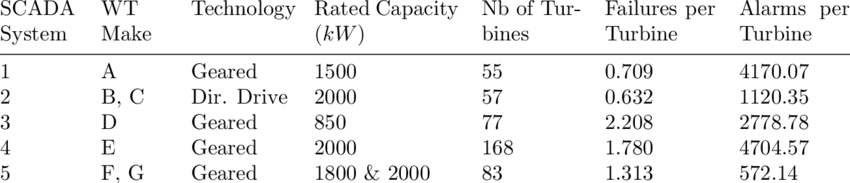
\includegraphics[scale=0.4]{SCADA_table}
	\decoRule
	\caption{Data used for the SCADA Alarms and Failure Analysis \cite{wind_turbine_failures}}
	\label{fig:SCADA_table}
\end{figure}

According to a study on wind turbine accidents \cite{wind_turbine_accidents}, there are 4 main categories of accidents.  These include transportation, construction, operation, and maintenance accidents, which can be caused by either nature, human error, or equipment failure.  According to the study, operation accidents are significantly more common than any other category of failures \cite{wind_turbine_failures}.  Most of the operation accidents (about 80\%) are caused by either equipment failures or nature events.  The detection method outlined in this document would hopefully be able to prevent many of the operation-based accidents, which are a majority of the turbine accidents.

\section{Tower Vibration Research}
Wind turbine tower vibrations are important to the health of turbines and have been studied before.  In one study, a nonlinear state estimation technique \cite{NSET_vibration_modeling} (NSET) is used to attempt to predict wind turbine failures.  This model uses SCADA data to relate different operating parameters to the health of the turbine.  Typically, many variables are used as inputs to determine turbine health and status because vibration alone isn't always sufficient \cite{NSET_vibration_modeling}.  When many variables are used, statistical model become significantly more complex and require large-scale optimization processes which is where machine learning models accel.

Most tower vibration analyses are empirically derived because of the stochastic nature of the wind speed and the amount of variables affecting the turbine.  Data-driven models \cite{data_driven_online_monitoring} are very common in the wind power space, especially with monitoring systems such as SCADA.

\section{Small turbine monitoring system}
As previously discussed, there are a lot of options for large-scale turbine monitoring, but they are expensive and difficult to implement and maintain because many of them need to be directly integrated with the turbine computer to collect the necessary data.  Small-scale turbine systems don't have all of the same requirements as the large-scale systems.  It is valuable to have a lightweight and inexpensive device that can monitor the health of a turbine without requiring direct integration to internal operation parameters.  Ideally, this device should be able to detect impending problems, halt operation, and notify the maintenance operator.

A small-turbine monitoring system would reduce the frequency of maintenance because it would only need to be checked when the system reports possible trouble.  It would also reduce the operation and maintenance cost by stopping all operations when there is a possible problem.  Because this device won't have access to internal operating parameters (such as generator power, internal temperature, rotor speed, wind speed, and wind direction), it will need to monitor the turbine vibrations, which can efficiently be done using accelerometers.  One common turbine problem is a rotor imbalance, caused by either blade damage, loose fasteners, or build-up material on the blades.  If the monitoring device can detect these imbalances, the turbine can be fixed before any additional damage is done.

Additionally, an ideal monitoring device would be wireless and battery-powered.  This means the processor should be very low-power and will need very efficient algorithms and data processing methods when acquiring data and making predictions.  This document will discuss various signal processing methods and their efficiencies, along with analyzing a few machine learning models for rotor imbalance predictions.




\chapter{Mathematical Model} % Main chapter title

\label{ch_math_model}

%----------------------------------------------------------------------------------------
%	SECTION 1
%----------------------------------------------------------------------------------------

\section{Assumptions/Problem Statement}

The turbine tower is modeled as a cantilever beam with a concentrated mass at the end.  The tower is the beam itself, and the nacelle is a concentrated mass at the end of the simplified beam.  The tower mass is condensed into an effective lump sum mass and added to the nacelle mass.  This allows the tower to be treated as a mass-less cantilever beam.

This problem is treated as forced vibration, where the forcing function is a periodic force caused from an eccentric mass on the rotor.  This eccentric mass represents an imbalance in the turbine, and will cause vibrations in the tower.   Figure \ref{fig:annotated_tower} shows the simplified wind turbine model with the applied forces. The cross-section of the tower is assumed to taper linearly from the base to the top.

\begin{figure}
	\centering
	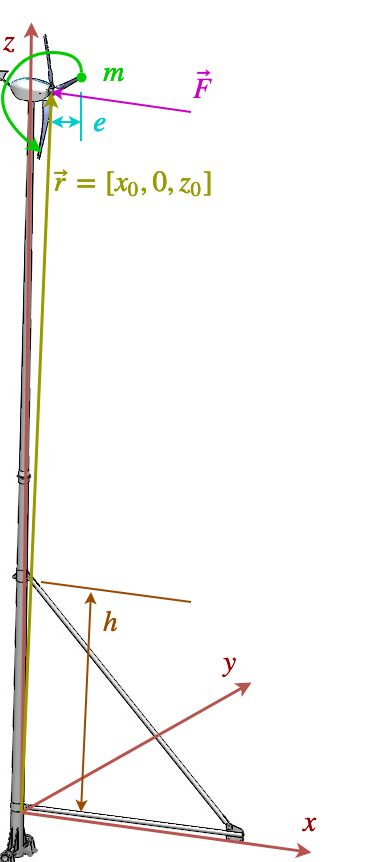
\includegraphics[scale=0.5]{annotated_tower}
	\decoRule
	\caption{The simplified wind turbine model showing the forces from an eccentric mass on the rotor.  This figure also shows the coordinate system that will be used for the tower analysis and is created using a Draw.io overlay on a SolidWorks model.}
	\label{fig:annotated_tower}
\end{figure}

%----------------------------------------------------------------------------------------
%	VARIABLE DEFINITIONS
%----------------------------------------------------------------------------------------

\section{Variable Definitions}

\begin{table}[] \label{t:variable_definitions}
\caption{Variable Definitions}
\vspace*{0.2in}
\begin{tabular}{|m{1in}|m{4in}|}
\hline
\rowcolor[HTML]{EFEFEF} 
\textbf{Variable} & \textbf{Description} \\ \hline
$\vec{F}_{original}$ & The original force applied to the end of the rotor due to an imbalance in the blades \\ \hline
$F_0$ & The magnitude of the force caused by the eccentric mass \\ \hline
$\omega$ & The rotational speed of the blades \\ \hline
$t$ & Time \\ \hline
$m$ & Eccentric mass \\ \hline
$e$ & Distance the eccentric mass is from the axis of rotation of the rotor \\ \hline
$\vec{M}$ & Moment that the eccentric force applies after the force is translated to the tower axis \\ \hline
$\vec{r}$ & The position vector for the top of the rotor with respect to the bottom of the turbine tower ($r=[x_0, 0, z_0]$) \\ \hline
$M_x$ & The moment function in the $x$-direction \\ \hline
$M_y$ & The moment function in the $y$-direction \\ \hline
$I_b$ & The area moment of inertia at the base of the tower \\ \hline
$I_t$ & The area moment of inertia at the top of the tower \\ \hline
$h$ & The distance from the base of the tower to the ginpole pin-joint on the tower \\ \hline
$E$ & Modulus of elasticity of the tower (steel) \\ \hline
$d_b$ & Diameter at the base of the tower \\ \hline
$d_t$ & Diameter at the top of the tower \\ \hline
\end{tabular}
\end{table}
\FloatBarrier



%----------------------------------------------------------------------------------------
%	CALCULATING TOWER VIBRATIONS
%----------------------------------------------------------------------------------------

\section{Calculating Tower Vibrations}

\subsection{Determining Effective Force}

An eccentric mass, $m$, on the rotor causes a force defined by the following equation:

\begin{equation} \label{eq:initial_force}
	\vec{F}(t) = 
		\begin{bmatrix}
			0 \\
			F_0\sin{(\omega t)} \\
			F_0\cos{(\omega t)}	
		\end{bmatrix}
\end{equation}

where

\begin{equation}
	F_0 = me\omega^2
\end{equation}

In order to treat the system as a cantilever beam, the force has to be acting in the center of the nacelle and on the same axis as the tower.  When the force vector (Equation \ref{eq:initial_force}) is translated to the axis of the tower, a moment needs to be introduced to account for the force vector translation:

\begin{equation} \label{eq:translated_moment}
	\vec{M} = \vec{r} \times \vec{F} = 
		\begin{bmatrix}
			- F_{0} z_{0} \sin{\left (\omega t \right )}\\
			- F_{0} x_{0} \cos{\left (\omega t \right )}\\
			F_{0} x_{0} \sin{\left (\omega t \right )}
		\end{bmatrix}
\end{equation}

The moment in (Equation \ref{eq:translated_moment}) creates an effective force at the top of the tower that needs to be added to the original force (Equation \ref{eq:initial_force}).  The moment about the $z$-axis is ignored because torsional effects on the tower are negligible when determining nacelle displacement.  This results in the following effective force on the top of the tower:

\begin{equation}\label{eq:effective_force}
	\vec{F}_{effective} = \vec{F}_{original} + \vec{F}_{moment}
\end{equation}
$$ 
	\vec{F}_{effective} = 
	\begin{bmatrix}0\\F_{0} \sin{\left (\omega t \right )}\\F_{0} \cos{\left (\omega t \right )}\end{bmatrix}
	+ \begin{bmatrix}- \frac{F_{0} x_{0}}{z_{0}} \cos{\left (\omega t \right )}\\ F_{0} \sin{\left (\omega t \right )}\\ 0\end{bmatrix}
$$

\begin{equation}
	\vec{F}_{effective} = 
		\left[\begin{matrix}- \frac{F_{0} x_{0}}{z_{0}} \cos{\left (\omega t \right )}\\2 F_{0} \sin{\left (\omega t \right )}\\F_{0} \cos{\left (\omega t \right )}\end{matrix}\right]
\end{equation}

%----------------------------------------------------------------------------------------
%	DETERMINING EFFECTIVE SPRING CONSTANT
%----------------------------------------------------------------------------------------
\subsection{Determining Effective Spring Constant}
The tower model has a different spring constant for the $x$ and $y$ directions.  In the $y$ direction, the ginpole has a negligible effect on the stiffness of the tower, so the tower acts as a tapered cantilever beam. 


%	Deriving the y-direction spring constant
%----------------------------------------------------------------------------------------
\subsubsection{Mathematical derivation of the $y$-direction spring constant, $K_y$}
Assuming the tower acts like a cantilever beam in this direction with a concentrated force at the end of the beam, the moment, $M_x(y)$ can be expressed as:

\begin{equation} \label{eq:moment}
	M_x(y) = F_{y}\,z-F_{y}\,z_{0}
\end{equation}

Because the beam is linearly tapered, the diameter, $d$, can be written as a function of tower height, $z_0$.

\begin{equation} \label{eq:diameter_eq}
	d(z) = d_{b}-\frac{z\,\left(d_{b}-d_{t}\right)}{z_{0}}
\end{equation}

$d_b$ is the diameter of the tower at the bottom, and $d_t$ is the diameter of the tower at the top.  The moment of inertia, assuming a hollow tube with thickness $t$, can be written as a function of $z$ using Equation \ref{eq:diameter_eq}.

\begin{align}
	I_y(z) &= \frac{\pi}{64}d^4 - \frac{\pi}{64}\left(d-2t \right)^4 \\
	I_y(z) &= \frac{\pi \,{\left(d_{b}-\frac{z\,\left(d_{b}-d_{t}\right)}{z_{0}}\right)}^4}{64}-\frac{\pi \,{\left(2\,t-d_{b}+\frac{z\,\left(d_{b}-d_{t}\right)}{z_{0}}\right)}^4}{64} \label{eq:y_moment_intertia}
\end{align}

The deflection of the beam can be calculated using the Euler–Bernoulli equation:

\begin{align}
	\frac{d^2 y_d}{dz^2} &= -\frac{M_x}{E\,I_y(z)} \\
	\frac{d^2 y_d}{dz^2} &= -\frac{F_{y}\,z-F_{y}\,z_{0}}{E\,\left(\frac{\pi \,{\left(d_{b}-\frac{z\,\left(d_{b}-d_{t}\right)}{z_{0}}\right)}^4}{64}-\frac{\pi \,{\left(2\,t-d_{b}+\frac{z\,\left(d_{b}-d_{t}\right)}{z_{0}}\right)}^4}{64}\right)}
 \label{eq:curvature_eq_y}
\end{align}

The slope of the beam, $\theta_y$, can be calculated by integrating Equation \ref{eq:curvature_eq_y}:

\begin{equation}
	\theta_y = \frac{dy_d}{dz} = \int{-\frac{F_{y}\,z-F_{y}\,z_{0}}{E\,\left(\frac{\pi \,{\left(d_{b}-\frac{z\,\left(d_{b}-d_{t}\right)}{z_{0}}\right)}^4}{64}-\frac{\pi \,{\left(2\,t-d_{b}+\frac{z\,\left(d_{b}-d_{t}\right)}{z_{0}}\right)}^4}{64}\right)}\,dz}
\end{equation}

Integrating the equation above results in the following equation for $\theta_y$:

\begin{align}
	\theta_y =\, &\frac{\ln\left(d_{b}\,z-d_{t}\,z-d_{b}\,z_{0}+t\,z_{0}\right)\,\left(8\,F_{y}\,d_{t}\,{z_{0}}^2-8\,F_{y}\,t\,{z_{0}}^2\right)}{E\,\pi \,{d_{b}}^2\,t^3-2\,E\,\pi \,d_{b}\,d_{t}\,t^3+E\,\pi \,{d_{t}}^2\,t^3} \nonumber \\
	&-\frac{4\,\ln\left(d_{b}\,z-d_{t}\,z-d_{b}\,z_{0}+t\,z_{0}\,\left(1-\mathrm{i}\right)\right)\,\left(F_{y}\,d_{t}\,{z_{0}}^2+F_{y}\,t\,{z_{0}}^2\,\left(-1+1{}\mathrm{i}\right)\right)}{E\,\pi \,{d_{b}}^2\,t^3-2\,E\,\pi \,d_{b}\,d_{t}\,t^3+E\,\pi \,{d_{t}}^2\,t^3} \nonumber \\
	&-\frac{4\,\ln\left(d_{b}\,z-d_{t}\,z-d_{b}\,z_{0}+t\,z_{0}\,\left(1+1{}\mathrm{i}\right)\right)\,\left(F_{y}\,d_{t}\,{z_{0}}^2+F_{y}\,t\,{z_{0}}^2\,\left(-1-\mathrm{i}\right)\right)}{E\,\pi \,{d_{b}}^2\,t^3-2\,E\,\pi \,d_{b}\,d_{t}\,t^3+E\,\pi \,{d_{t}}^2\,t^3} + C_{y1}
\end{align}


The tower is fixed at the base (no translation or rotation about the $x$-axis), so the slope at $z=0$ is $\theta=0$.  Using this boundary condition, $C_{y1}$ can be determined:
\begin{align}
	C_{y1} = -\frac{4\,F_{y}\,{z_{0}}^2\,Q_1(z)}{E\,t^3\,\pi \,{\left(d_{b}-d_{t}\right)}^2}
\end{align}

where, 
\begin{align*}
	Q_1(z) =\, &2\,d_{t}\,\ln\left(-z_{0}\,\left(d_{b}-t\right)\right)-d_{t}\,\ln\left(-z_{0}\,\left(d_{b}+t\,\left(-1-\mathrm{i}\right)\right)\right) \\
	&-d_{t}\,\ln\left(-z_{0}\,\left(d_{b}+t\,\left(-1+1{}\mathrm{i}\right)\right)\right)-2\,t\,\ln\left(-z_{0}\,\left(d_{b}-t\right)\right) \\
	&+t\,\ln\left(-z_{0}\,\left(d_{b}+t\,\left(-1-\mathrm{i}\right)\right)\right)\,\left(1+1{}\mathrm{i}\right) \\
	&+t\,\ln\left(-z_{0}\,\left(d_{b}+t\,\left(-1+1{}\mathrm{i}\right)\right)\right)\,\left(1-\mathrm{i}\right)
\end{align*}

This results in the following slope equation:

\begin{align} \label{eq:theta_analytic}
	\theta_y = \frac{4\,F_{y}\,{z_{0}}^2\,Q_2(z)}{E\,t^3\,\pi \,{\left(d_{b}-d_{t}\right)}^2} + C_{y1}
\end{align}

where,
\begin{align*}
	Q_2(z) =\, &2\,d_{t}\,\ln\left(d_{b}\,z-d_{t}\,z-d_{b}\,z_{0}+t\,z_{0}\right) \\
	&-d_{t}\,\ln\left(d_{b}\,z-d_{t}\,z-d_{b}\,z_{0}+t\,z_{0}\,\left(1-\mathrm{i}\right)\right) \\
	&-d_{t}\,\ln\left(d_{b}\,z-d_{t}\,z-d_{b}\,z_{0}+t\,z_{0}\,\left(1+1{}\mathrm{i}\right)\right) \\
	&-2\,d_{t}\,\ln\left(-z_{0}\,\left(d_{b}-t\right)\right)+d_{t}\,\ln\left(-z_{0}\,\left(d_{b}+t\,\left(-1-\mathrm{i}\right)\right)\right) \\
	&+d_{t}\,\ln\left(-z_{0}\,\left(d_{b}+t\,\left(-1+1{}\mathrm{i}\right)\right)\right) \\
	&-2\,t\,\ln\left(d_{b}\,z-d_{t}\,z-d_{b}\,z_{0}+t\,z_{0}\right) \\
	&+t\,\ln\left(d_{b}\,z-d_{t}\,z-d_{b}\,z_{0}+t\,z_{0}\,\left(1-\mathrm{i}\right)\right)\,\left(1-\mathrm{i}\right) \\
	&+t\,\ln\left(d_{b}\,z-d_{t}\,z-d_{b}\,z_{0}+t\,z_{0}\,\left(1+1{}\mathrm{i}\right)\right)\,\left(1+1{}\mathrm{i}\right) \\
	&+2\,t\,\ln\left(-z_{0}\,\left(d_{b}-t\right)\right)+t\,\ln\left(-z_{0}\,\left(d_{b}+t\,\left(-1-\mathrm{i}\right)\right)\right)\,\left(-1-\mathrm{i}\right) \\
	&+t\,\ln\left(-z_{0}\,\left(d_{b}+t\,\left(-1+1{}\mathrm{i}\right)\right)\right)\,\left(-1+1{}\mathrm{i}\right)
\end{align*}

At this point, it has become clear that an analytic solution for the spring constant is not practical.  Integrating the slope equation (Equation \ref{eq:theta_analytic}) would produce the deflection equation; however this integral become extremely complicated.  A cleaner option is to calculate the spring constants numerically.

\subsubsection{Numerical calculation of the $y$-direction spring constant, $K_y$}
To determine the spring constant numerically, a vector of $z$ values must be created to be used in the numerical integration. 

To calculate the slope of the tower, $\theta$, the curvature equation needs to be numerically integrated:

\begin{equation}
	\theta(z) = \int_0^{z_0}{\frac{-M(z)}{E\,I(z)}\,dz}
\end{equation}

The applied force, $F_y$, in the moment equation (Equation \ref{eq:moment}) can be factored out because it is not a function of $z$.  This results in the following equation for the slope:

\begin{equation} \label{eq:theta_integral_exact}
	\theta(z) = \frac{F_y}{E} \int_0^{z_0}{\frac{z_0-z}{I(z)}\,dz}
\end{equation}

The integral in Equation \ref{eq:theta_integral_exact} can be approximated by a sum of $n$ elements and calculated numerically.

\begin{equation} \label{eq:theta_integral_approx}
	\theta(z) = \frac{F_y}{E} \sum_{i=0}^{n}{\frac{z_0-z_i}{I(z_i)}\,\Delta z_i}
\end{equation}

Equation \ref{eq:theta_integral_approx} is a much simpler method for calculating the beam slope compared to the analytic solution shown in Equation \ref{eq:theta_analytic}.  The deflection of the tower, $y_d$, can be calculated by integrating the slope equation.

\begin{equation}
	y_d = \int_{0}^{z_0}{\theta(z)\,dz} = \int_{0}^{z_0}{\left(\frac{F_y}{E} \sum_{i=0}^{n}{\frac{z_0-z_i}{I(z_i)}\,\Delta z_i}\right)dz}
\end{equation}

The above equation can be numerically approximated with a summation of $m$ elements as follows:

\begin{align}
	y_d &= \sum_{j=0}^{m}{\left(\frac{F_y}{E} \sum_{i=0}^{n}{\frac{z_0-z_{ij}}{I(z_{ij})}\,\Delta z_i}\right) \Delta z_j} \\
	y_d &= \frac{F_y}{E}\sum_{j=0}^{m}{\sum_{i=0}^{n}{\frac{z_0-z_{ij}}{I(z_{ij})}\,\Delta z_i} \Delta z_j} \label{eq:deflection_equation_sum}
\end{align}

To determine the spring constant, the deflection equation should be rewritten in the form, $F=-kx$, which in this case is:
\begin{align}
	F_y &= -k_y \, y_d \\
	F_y &= \frac{E}{\sum_{j=0}^{m}{\sum_{i=0}^{n}{\frac{z_{ij}-z_0}{I(z_{ij})}\,\Delta z_i} \Delta z_j}} \, y_d \label{eq:Fy_numerical}
\end{align}

From Equation \ref{eq:Fy_numerical}, is can be seen that the spring constant is:
\begin{equation} \label{eq:ky}
	k_y = \frac{E}{\sum_{j=0}^{m}{\sum_{i=0}^{n}{\frac{z_{ij}-z_0}{I(z_{ij})}\,\Delta z_i} \Delta z_j}}
\end{equation}


\begin{table}[]
\caption{Calculated spring constant and natural frequency for the $y$-direction vibration.} \label{t:ky_values}
\begin{center}
\begin{tabular}{|m{1in}|m{1in}|m{1in}|m{1in}|m{1in}|}
\rowcolor[HTML]{EFEFEF} 
\hline
\textbf{Parameter} & \textbf{Constant Top Area} & \textbf{Tapered Beam} & \textbf{Constant Bottom Area} & \textbf{FEA value} \\ \hline
$k_y$ & 1283 N/m & 8966 N/m & 16213 N/m & 8159 N/m \\  \hline
$f_y$ & 0.34 Hz & 0.61 Hz & 1.1 Hz & 0.58 Hz\\ \hline
\end{tabular}
\end{center}
\end{table}

Table \ref{t:ky_values} shows the calculated spring constant values and natural frequencies in the $y$-direction for the turbine parameters.  The constant top area value is the spring constant calculated assuming a uniform circular cross-section beam with a profile equal to the top of the tower.  The constant bottom area value is the spring constant calculated assuming a uniform circular cross-section beam with a profile equal to the bottom of the tower.  The FEA values are derived in Tom Gwon's analysis \cite{Gwon_paper}, although it is unclear whether these values apply for the $y$ or $x$ direction.  The tapered beam calculation is performed in MATLAB using the following code (with turbine parameters listed in Table \ref{t:MATLAB_ky_variables}):

\begin{lstlisting}
z = linspace(0, z_0, 1000); % [m] Create the vector of z values
M_F = (z - z_0); % [m] The moment equation with respect to the applied force (M/F)
d_F = d_b - z*(d_b-d_t)/z_0; % [m] The diameter as a function of height
I = pi/64*d.^4 - (pi/64)*(d-2*t).^4; % [m^4] The moment of inertia
v_F = -M_F ./ (E*I); % [s^2/m^2/kg] The curvature equation
theta_F = cumtrapz(z, v_F); % [s^2/m/kg] The slope equation
y_F = cumtrapz(z, theta_F); % [m/N] The displacement with respect to force
ky = 1 ./ y_F(end); % [N/m] Spring constant
\end{lstlisting}
\FloatBarrier


\begin{table}[]
\caption{Turbine parameters used in the MATLAB analysis for calculating $k_y$}
\label{t:MATLAB_ky_variables}
\vspace*{0.2in}
\begin{tabular}{|m{1in}|m{1in}|m{4in}|}
\hline
\rowcolor[HTML]{EFEFEF} 
\textbf{Variable} & \textbf{Value} & \textbf{Description} \\ \hline
$z_0$ & 70 ft & The total height of the tower \\ \hline
$d_b$ & 20 in & The diameter of the bottom of the tower \\ \hline
$d_t$ & 8.7 in & The diameter of the top of the tower \\ \hline
$E$ & 30 Mpsi & The modulus of elasticity for ASTM A572 Grade-50 Steel \\ \hline
$t$ & 0.2 in & The thickness of the turbine tower tube \\ \hline
\end{tabular}
\end{table}

The intermediate variables from the MATLAB calculation are shown in Figure  \ref{fig:ky_MATLAB_plot}.  The curvature, slope, and displacement are all with respect to force, since it cancels out of the equation and is not used.  The spring constant is calculated by taking the inverse of the displacement/force curve at the largest $z$ value.  These plots were created using a $z$-vector of 1000 elements.

\begin{figure}
	\centering
	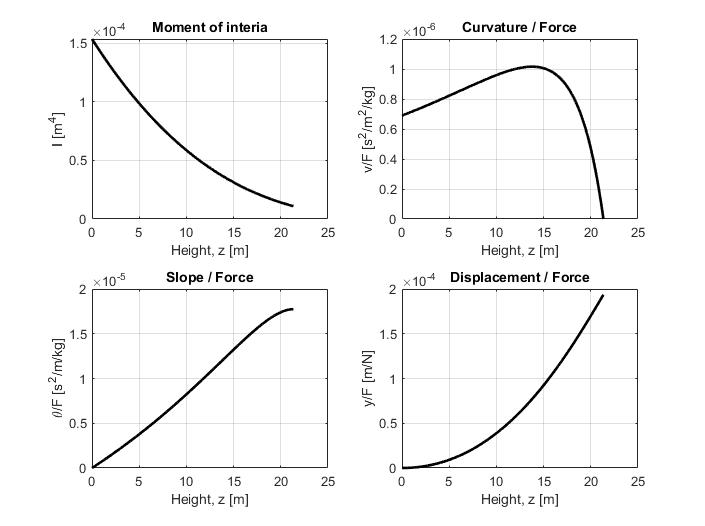
\includegraphics[scale=0.7]{ky_MATLAB_plot}
	\decoRule
	\caption{The intermediate variables from the numerical spring constant calculation in MATLAB.}
	\label{fig:ky_MATLAB_plot}
\end{figure}
\FloatBarrier


%----------------------------------------------------------------------------------------
%	DETERMINING EFFECTIVE MASS
%----------------------------------------------------------------------------------------

\subsection{Determining Effective Mass}
The cantilever beam (Figure \ref{fig:cantilever_beam}) can be simplified to a massless beam with all of the mass concentrated at the end of the beam.

% Figure for the cantilever beam
\begin{figure}
	\centering
	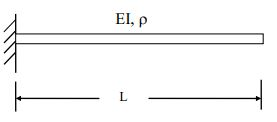
\includegraphics[scale=1]{cantilever_beam}
	\decoRule
	\caption{A cantilever beam model \cite{cantilever_beam_ref}}
	\label{fig:cantilever_beam}
\end{figure}

As shown in Figure \ref{fig:ky_MATLAB_plot}, the deflection at any point on the beam, $y(z)$ can be calculated numerically.  The normalized deflection, $y_n(z)$ can be calculated by dividing this equation by the maximum deflection at the free end, $z_0$ (Equation \ref{eq:normalized_deflection}).  This allows the deflection equation to be rewritten in terms of the normalized deflection (Equation \ref{eq:deflection_w_normalization}).
\begin{align}
	y_n(z) &= \frac{y(z)}{y(z_0)} \label{eq:normalized_deflection} \\
	y(z) &= y_n(z) \cdot y(z_0) = y_n(z) \cdot y_{max} \label{eq:deflection_w_normalization} \\
\end{align}

The velocity of the beam at point $z$ can be calculated by taking the derivative of the deflection equation (Equation \ref{eq:deflection_w_normalization}).  The velocity of the beam is shown in Equation \ref{eq:beam_velocity}.
\begin{equation} \label{eq:beam_velocity}
	v(z) = y_n(z) \cdot v_{max}
\end{equation}

The kinetic energy, $dE_k$, of the beam at a single point, $x$, can be calculated as shown in Equation \ref{eq:beam_ke}.
\begin{align}
	dE_k &= \frac{1}{2} m v^2 \nonumber \\
	dE_k &= \frac{1}{2} \left(\rho A(z) dz\right) \left(y_n(z) v_{max}\right)^2  \label{eq:beam_ke}
\end{align}

Using Equation \ref{eq:beam_ke}, the total kinetic energy of the beam can be found by integrating $dE_k$, as shown in Equation \ref{eq:beam_ke_total}.
\begin{align}
	E_k &= \int_{0}^{z_0}{dE_k} \\
	E_k &= \int_{0}^{z_0}{\left(\frac{1}{2} \rho A(z) \left(y_n(z) v_{max}\right)^2 dz \right)} \\
	E_k &= \frac{1}{2} \rho v_{max}^2 \int_{0}^{z_0}{\left(A(z) y_n^2(z) dz \right)} \label{eq:beam_ke_total}
\end{align}

The effective mass of the beam can be calculated by examining Equation \ref{eq:beam_ke_total} and comparing to the standard format, $E=\frac{1}{2}mv^2$.  Equation \ref{eq:effective_mass_integral} shows the resulting effective mass.
\begin{equation} \label{eq:effective_mass_integral}
	m_{eff} = \rho \int_{0}^{z_0}{\left(A(z) y_n^2(z) dz \right)}
\end{equation}

The deflection from Equation \ref{eq:deflection_equation_sum} can be substituted into Equation \ref{eq:effective_mass_integral}.  Additionally, the integral can be converted to a numerical sum as shown in Equation \ref{eq:m_eff_sum}.
\begin{equation} \label{eq:m_eff_sum}
	m_{eff} = \rho \sum_{k=0}^{p}{\left(A(z_p) y_n^2(z_p) \Delta z \right)}
\end{equation}

Numerically calculating $m_{eff}$ using MATLAB, results in a value of $m_{eff}=140 \units{kg}$.

The total effective mass at the top of the tower, $m_{eff,total}$ is as follows:
\begin{align}
	m_{eff,total} &= m_{nacelle} + m_{eff} \\
	m_{eff,total} &= 474 \units{kg} + 140 \units{kg} = 614 \units{kg} \label{eq:total_effective_mass}
\end{align}

The mass in Equation \ref{eq:total_effective_mass} is the lumped sum used to calculate the  parameters in Table \ref{t:ky_values} and create the turbine tower model.

\subsection{Developing State Space Equations}
Vibrations in the $x$ and $y$ directions can be split up into 2 independent 2nd order differential equations:
\begin{align}
	\ddot{x} + \frac{C_x}{m} \dot{x} + \frac{k_x}{m} x = \frac{1}{m} F_x(t) \\
	\ddot{y} + \frac{C_y}{m} \dot{y} + \frac{k_y}{m} x = \frac{1}{m} F_y(t)
\end{align}

These equations can be converted to state space form:
\begin{align}
	&\bm{\dot{x}} = \bm{A_x} \bm{x} + \bm{B_x} F_x(t) \\
	&x = \bm{C_x} \bm{x} + \bm{D_x} F_x(t) \\
	&\bm{\dot{y}} = \bm{A_y} \bm{y} + \bm{B_y} F_y(t) \\
	&y = \bm{C_y} \bm{y} + \bm{D_y} F_y(t)
\end{align}

Where the full equations are written out as follows:
\begin{align}
	\begin{bmatrix}
		\dot{x}_1 \\
		\dot{x}_2
	\end{bmatrix} = 		
	\left[\begin{matrix}0 & 1\\- \frac{k_{x}}{m} & - \frac{C_{x}}{m}\end{matrix}\right]
	\left[\begin{matrix}x_{1} \\ x_{2}\end{matrix}\right] +
	\left[\begin{matrix}0 \\ \frac{1}{m}\end{matrix}\right] \cdot F_x(t)\\
	x=
	\begin{bmatrix}
		1 & 0
	\end{bmatrix}
	\begin{bmatrix}
		x_1 \\ x_2		
	\end{bmatrix} + 0 \cdot F_x(t)
\end{align}

\begin{align}
	\begin{bmatrix}
		\dot{y}_1 \\
		\dot{y}_2
	\end{bmatrix} = 		
	\left[\begin{matrix}0 & 1\\- \frac{k_{y}}{m} & - \frac{C_{y}}{m}\end{matrix}\right]
	\left[\begin{matrix}y_{1} \\ y_{2}\end{matrix}\right] +
	\left[\begin{matrix}0 \\ \frac{1}{m}\end{matrix}\right] \cdot F_y(t)\\	
	y=
	\begin{bmatrix}
		1 & 0
	\end{bmatrix}
	\begin{bmatrix}
		y_1 \\ y_2		
	\end{bmatrix} + 0 \cdot F_y(t)	
\end{align}

These equations are for a simple cantilever model with a lumped mass at the end of the beam (lumped mass accounts for nacelle and tower mass).  The resulting natural frequency from this model matches the ABAQUS FEA results from Gwon's paper \cite{Gwon_paper}.  A comparison between the resulting natural frequency from this model and the ABAQUS FEA results in Gwon's analysis \cite{Gwon_paper} can be seen in Table \ref{t:ky_values}.
\chapter{Digital Signal Processing Model} % Main chapter title

\label{ch_dsp_model} 

% Model Block Diagram -------------------------------------------------
\section{Model Block Diagram}
The blade imbalance detection is simulated using MATLAB/Simulink.  Figure \ref{fig:LIA_block_diagram} shows the block diagram for a method of imbalance detection where the rotor frequency is known.  This is an accurate method, but requires the information from an encoder on the shaft or an accurate phase-locked loop (PLL) controller.  

The force due to an imbalance is given in Equation \ref{eq:initial_force}.  It is a periodic function with the same frequency as the rotor and is proportional to the effective imbalance mass, $m$.  The variable forcing function is the input for the lumped parameter turbine tower state space model. These vibrations are then read by an acceleration sensor with a sampling rate of 100 Hz.  The frequency of interest is demodulated using a lock-in amplifier or DFT, which should result in the acceleration from only the imbalance.  The acceleration at the top of the tower should have higher intensity vibrations at the rotor frequency when there is an imbalance in the blades (causing an eccentric mass).

\begin{figure}
	\centering
	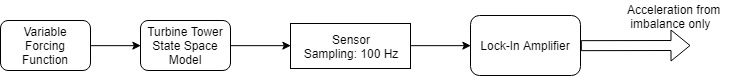
\includegraphics[scale=0.6]{LIA_block_diagram}
	\decoRule
	\caption{A block diagram showing the lock-in amplifier and the turbine tower simulation.}
	\label{fig:LIA_block_diagram}
\end{figure}

%----------------------------------------------------------------------------------------

\section{Processing the data}

This paper describes a few ways to process the acceleration data from the turbine tower.  One method relies on accurate frequency information to precisely demodulate the signal at the rotor frequency.  An alternative method is to lock onto the strong frequency vibration of the tower using a phased-lock loop controller.  Finally, a discrete Fourier transform can be calculated to transform the time domain data to the frequency domain.  There are various ways to make this process more efficient, including zoom FFTs and the Goertzel algorithm.

The simulation and turbine tower state space model produce displacements shown in Figure \ref{fig:simulated_sensor_reading}.  The same simulation data is shown in the frequency domain  in Figure \ref{fig:sim_FFT_200RPM}.  From the frequency domain, it can be seen that there is resonance at 0.84 Hz (the natural frequency of the tower in the $x$-direction).  Additionally, there is an excitation at the rotor frequency that has a magnitude proportional to the amount of mass at the end of the blade.  This simplified linear model produces an displacement signal that can be represented by the sum of sines as shown in Equation \ref{eq:sum_of_sines} (this can be seen in Figure \ref{fig:simulated_sensor_reading}).
\begin{equation} \label{eq:sum_of_sines}
	y = C_1 \sin{(\omega_n t + \phi_1)} + C_2 \sin{(\omega_{drive} t + \phi_2)}
\end{equation}

The first method for processing the acceleration data utilizes lock-in amplifier to translate the data in the frequency domain.  This new data, with the rotor frequency shifted to 0 Hz, is filtered and results in a DC acceleration that should be proportional to the imbalance mass.  The second method utilizes a zoom FFT, which provides higher resolution than a typical FFT in the bandwidth of interest.  The third method uses a Goertzel algorithm to calculate the bin of interest in the DFT.

\begin{figure}
	\centering
	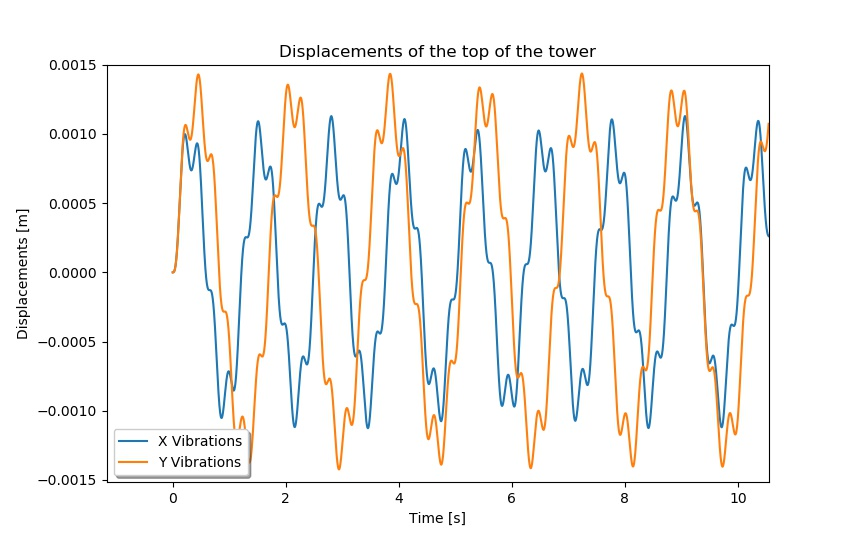
\includegraphics[scale=0.6]{simulated_sensor_reading}
	\decoRule
	\caption{The simulated displacement for a rotor imbalance at 230 RPM.  The imbalance mass is placed at the end of the blade, which causes accelerations and displacements at the top of the tower.}
	\label{fig:simulated_sensor_reading}
\end{figure}

\begin{figure}
	\centering
	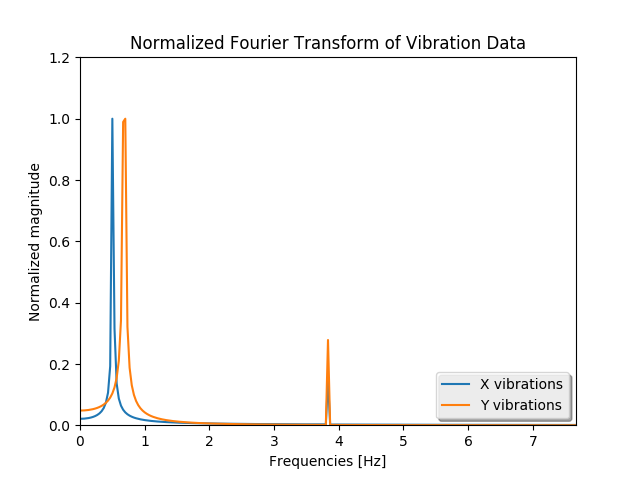
\includegraphics[scale=0.6]{sim_FFT_200RPM}
	\decoRule
	\caption{This figure shows the simulated displacement data in the frequency domain.  The rotor frequency is 230 RPM in this simulation}
	\label{fig:sim_FFT_200RPM}
\end{figure}

\subsection{DFT review}
A Discrete Fourier Transform (DFT) converts a signal from the time domain to the frequency domain.  Typically, this is performed with using the Fast Fourier Transform (FFT) algorithm, which is an efficient method for calculating the DFT.  The DFT is defined by the formula in Equation \ref{eq:dft_definition} \cite{wiki_DFT}.
\begin{equation} \label{eq:dft_definition}
	X_k = \sum_{n=0}^{N-1}{x_n \cdot e^{-\frac{i 2 \pi}{N} k n}}
\end{equation}

$\vec{x}$ is the original signal in the time domain with $N$ elements, and $\vec{X}$ is the signal in the frequency domain with $N$ elements.  Equation \ref{eq:dft_definition} can be rewritten using Euler's formula to show DFT equation in terms of sine and cosine values (this is important for understanding the lock-in amplifier in a future section).  Equation \ref{eq:dft_euler} shows the new expression for the DFT equation.
\begin{equation} \label{eq:dft_euler}
	X_k = \sum_{n=0}^{N-1}{x_n \cdot \left[ \cos{\left(\frac{2 \pi k n}{N}\right)} - j \sin{\left(\frac{2 \pi k n}{N}\right)} \right]}
\end{equation}

From Equation \ref{eq:dft_euler}, it can be seen that the DFT can be calculated by mixing the signal, $\vec{x}$, with a sine and cosine signal and summing the result for each frequency.  The DFT equation can be further rewritten using vector notation as in Equation \ref{eq:dft_vector} and defining some reference vectors.  This equation shows that the DFT of a signal is an imaginary vector that can be created from the dot products of the original signal and some reference sine and cosine signals.
\begin{align}
	\vec{n}_r &= 
		\begin{bmatrix}
			0/N \\
			1/N \\
			2/N \\
			\vdots \\
			(N-1)/N	
		 \end{bmatrix} \\
	\vec{r}_{sin} &= \sin{\left(2 \pi k \vec{n}_r\right)} \\
	\vec{r}_{cos} &= \cos{\left(2 \pi k \vec{n}_r\right)} \\
	X_k &= \vec{x}^T \cdot \vec{r}_{cos} - j \vec{x}^T \cdot \vec{r}_{sin}  \label{eq:dft_vector}
\end{align}

Another way of looking at the DFT (from the form in Equation \ref{eq:dft_vector}) is as a time domain convolution with a low pass filter.  The summation (shown explicitly in the form from Equation \ref{eq:dft_euler}) acts as a simple finite impulse response (FIR) decimation filter with unity coefficients and a decimation rate of $d=N$, commonly known as an averaging filter.  When thinking about the DFT in this way, some possible optimization methods start to become clear.  For example, we may not need to calculate the frequency component for every $k$th element in $\vec{X}$, and we may choose to use a better filter that has stronger attenuation at higher frequencies.  This is the basis for the lock-in amplifier design described in the next section.


\subsection{Lock-In Amplifier}

A lock-in amplifier is used to measure AC signals in particularly noisy environments (Figure \ref{fig:LIA}).  It works by multiplying the noisy signal by a reference signal created by an internal oscillator.  By using 2 reference signals out of phase, the real and imaginary parts of the signal at the specified carrier frequency can be calculated\cite{LIA_document}.  Let's say there is an unknown sinusoidal signal with high frequency noise ($\omega_2 >> \omega_1$):
\begin{equation}
	y = A \,\sin{(\omega_1 \, t)} + B\,\sin{(\omega_2 \, t)}
\end{equation}

The amplitude of the signal, $A$, can be determined by multiplying the signal, $y$, by a reference signal with the same frequency as $\omega_1$ and filtering:
\begin{align}
	y \cdot \sin{(\omega_1 \, t)} &= \, \left[A \,\sin{(\omega_1 \, t)} + B\,\sin{(\omega_2 \, t)}\right] \, \sin{(\omega_1\,t)} \label{eq:sine_LIA}\\
	&=A\,\sin^2{(\omega_1\,t)} + B\,\sin{(\omega_1\,t)}\,\sin{(\omega_2\,t)} \\
	&=A\left(\frac{1}{2} - \frac{1}{2}\,\cos{(2\,\omega_1\,t)}\right) + B\,\sin{(\omega_1\,t)}\,\sin{(\omega_2\,t)} \label{eq:LIA_equation}
\end{align}

Note that Equation \ref{eq:sine_LIA} resembles the imaginary part of the standard DFT equation (Equation \ref{eq:dft_euler}), where the input signal is multiplied by a sine wave at a set reference frequency.

A filter is applied to Equation \ref{eq:LIA_equation} (similar to the summation filter used in Equation \ref{eq:dft_euler}), with a cutoff frequency that is smaller than $\omega_1$.  This results in all terms approaching zero, except for $\frac{A}{2}$, which can be calculated and solved for $A$ to achieve the magnitude of the frequency component at $\omega_1$.  To calculate the magnitude and phase of the signal $y$, it must be multiplied by a reference sine signal (as in Equation \ref{eq:sine_LIA}) and a reference cosine signal.  The following equation shows the result of the mixing step (phase-sensitive detection) in the lock-in amplifier:
\begin{equation} \label{eq:LIA_mixing}
	Y = X \cos{(\omega t)} + j X \sin{(\omega t)}
\end{equation}

where $X$ is the noisy AC signal and $Y$ is the signal that is fed into a filter to remove any unwanted frequency components at $\omega_1$ and $2 \omega_1$ and produce a signal, $Y_{filtered}$ that only contains the DC component:
\begin{equation}
	Y_{filtered} = \frac{A_{real}}{2} + j \frac{A_{imaginary}}{2}
\end{equation}

\begin{figure}
	\centering
	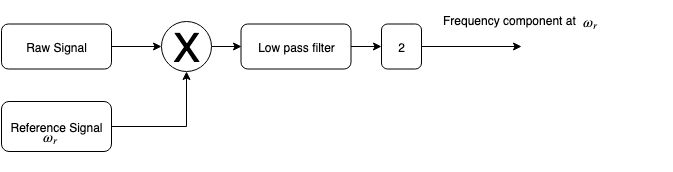
\includegraphics[scale=0.7]{LIA}
	\decoRule
	\caption{A block diagram showing the details of a lock-in amplifier \cite{LIA_fig}.  This figure was created with Draw.io.}
	\label{fig:LIA}
\end{figure}

Using the lock in amplifier tuned to a constant frequency, Figure \ref{fig:200_RPM_LIA_output_sim} shows the resulting output.  This shows that an imbalance can be detected by measuring the output of a lock-in amplifier that is tuned to the frequency of the turbine rotor.  When the acceleration data is treated as an AM signal, with the carrier frequency equal to the rotor frequency, the acceleration due to the rotation of the blades can be identified.  This acceleration is directly related to the mass at the end of the blade, and should be a constant value (as long as the rotor frequency is accurately known).

Lock-in amplifiers are typically used when the frequency is relatively stable and the signal-to-noise ratio is low.  For this application, the rotor frequency can change, which may not give the LIA filters enough time to settle.  If there is a very stable and accurate rotor speed controller, this method would be ideal because it extracts the signal of interest despite the high noise and distortions in the measurement.

\begin{figure}
	\centering
	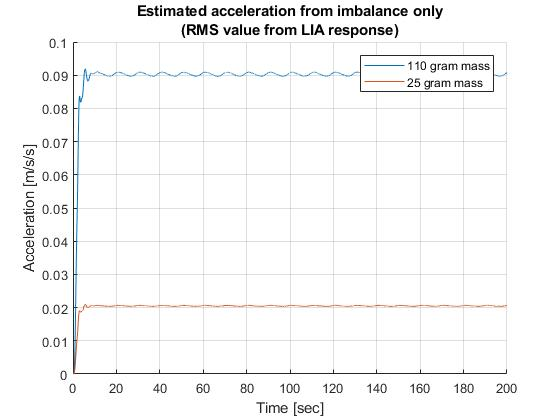
\includegraphics[scale=0.7]{200_RPM_LIA_output_sim}
	\decoRule
	\caption{The output of the lock-in amplifier from the simulated data shown in Figure \ref{fig:simulated_sensor_reading}}
	\label{fig:200_RPM_LIA_output_sim}
\end{figure}

\subsection{Identifying the rotor frequency from the tower accelerations}
If the rotor frequency cannot be measured directly it is possible to obtain the frequency indirectly from the acceleration data.  A phase-locked loop is a control system that minimizes the phase between to signals.  As the phase error is driven to zero, the output signal frequency approaches the input signal's frequency.  Phase-locked loops (PLLs) are commonly used in telecommunications where the frequency of a noisy signal can be recreated with an internal oscillator that locks on to the frequency of the noisy signal.  Figure \ref{fig:PLL_diagram} shows a block diagram of the PLL implementation with tower acceleration data as the input.

The first stage of the frequency detection is a narrow bandpass filter to get rid of high frequency noise and natural frequency resonance of the tower.  This is multiplied by an internal oscillator that starts at an arbitrary frequency (a guess that is close to the actual frequency, but not necessarily accurate).  This signal is passed through a lowpass filter to provide a steady phase error.  The phase error is driven to 0 using a PID controller.  This outputs the correct frequency of the signal that is then fed back and multiplied with the input signal.

One of the problems with a phase-locked loop is the PID controller gains depend on the amplitude of the signal, which changes depending on the amount of imbalance and rotor frequency.  The simplest approach to this would be to normalize the accelerations with the expected frequency.  This, however, is not perfect and doesn't account for the acceleration variation due to different eccentric masses.  A better solution would be to use a simple envelope detector to determine the amplitude of signal.  The accelerations can be divided by the output of the envelope detector to normalize the signal.  Figure \ref{fig:envelope_detector} shows an example of a simple envelope detector\cite{envelope_detector_ref}.  The low-pass filter in the envelope detector can be designed based on the desired accuracy.  For high computational efficiency, an averaging filter can be used because it minimizes the amount of multiply operations, and reduces the filter calculation to summations only.

\begin{figure}
	\centering
	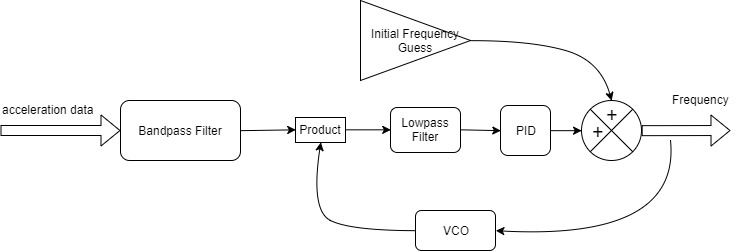
\includegraphics[scale=0.5]{PLL_diagram}
	\decoRule
	\caption{The block diagram of a phase-locked loop implementation when detecting rotor frequencies from acceleration measurements \cite{embedded_zoom_fft}.  This diagram was created with Draw.io \cite{draw_io}.}
	\label{fig:PLL_diagram}
\end{figure}

\begin{figure}
	\centering
	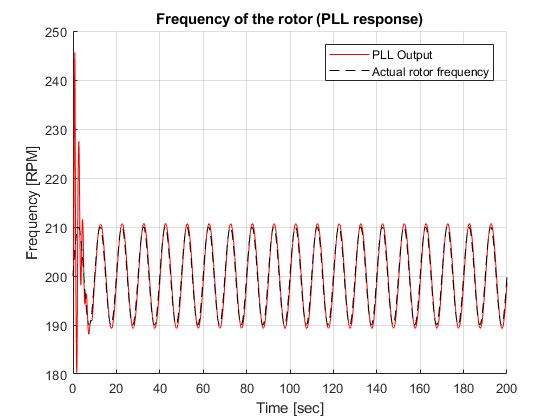
\includegraphics[scale=0.5]{PLL_simulation}
	\decoRule
	\caption{The output of the PLL  when detecting frequency from the data shown in Figure \ref{fig:simulated_sensor_reading}.  The frequency of the input data oscillates from 190 RPM to 210 RPM to simulate a real turbine controller that may oscillate between frequencies.}
	\label{fig:PLL_simulation}
\end{figure}

\begin{figure}
	\centering
	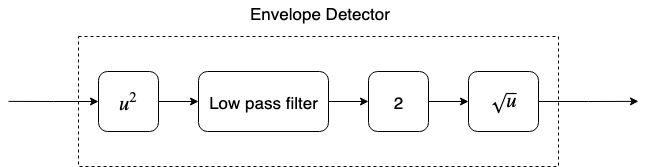
\includegraphics[scale=0.5]{envelope_detector}
	\decoRule
	\caption{A block diagram for a simple envelope detector.  The signal is first squared and multiplied by a gain of 2.  This signal (which should be entirely positive) is sent through a lowpass filter to remove the high frequency information.  The lowpass filter needs to reject $2f$, which is the resulting frequency when a signal with frequency, $f$ is squared.  The square root of the resulting signal produces the the amplitude of the signal.  This figure was created with Draw.io.}
	\label{fig:envelope_detector}
\end{figure}

\subsection{Zoom FFT}
A very powerful method for reducing the computational cost of the FFT calculation is to use a Zoom FFT.  If the imbalance detection device contains a low-power processor, it will be able to run for a long time off of a battery.  This also means that the processor could be much slower than an alternative high-power processor.  A Zoom FFT will significantly reduce the computational load on the processor, allowing the low-power processor to sufficiently calculate the frequency spectrum of the input signal.

One of the main tradeoffs for the reduced computational load, is a reduced frequency spectrum range.  For example, a set of 1024 data points sampled at $F_s$, will produce a frequency spectrum from $0$ to $F_s/2$ using the standard FFT.  A zoom FFT with a decimation rate of $D=10$ can produce a frequency spectrum with a range of $F_s/20$ at 1/10th the computational cost.

If the frequency of the rotor is not precisely known, then a lock-in amplifier is difficult to implement.  In order to detect excitation at the rotor frequency, the time-domain data can be transformed into the frequency domain.  A discrete Fourier transform (DFT) is the frequency domain representation of a sampled signal; however, can be slow and difficult to calculate on a microcontroller.

To efficiently calculate the Fourier transform, the DFT matrix can be factored and the complexity reduced from $O(n^2)$ to $O(n \log{n})$.  This efficient algorithm is called the fast Fourier transform (FFT).  Despite being much more efficient than the standard DFT, a generic FFT is still inefficient for this application because most of the frequency data occurs outside the bandwidth of interest and is thrown away.  This can be fixed by applying a zoom FFT algorithm.

The zoom FFT consists of 4 main steps.  First the data is convoluted with a reference signal in the time domain (translated in the frequency domain) to shift a center frequency, $F_c$, to 0 Hz.  Second, a lowpass filter prevents aliasing when sampling at a lower sample rate.  An infinite impulse response (IIR) filter can be used for simplicity; however, the phase information of the signal is lost.  To solve this, a finite impulse response (FIR) filter can be used.  FIR filters are more complicated but most have a flat phase response, ensuring the filter output retains the original phase information.  Typically, discrete FIR filters are applied in various 2-stage filters for simplicity.  Third, the data is decimated (re-sampled at a lower rate). Finally, the decimated data is passed through a FFT algorithm that produces a frequency spectrum in the specified bandwidth.  Since the frequency range of the zoom FFT is much smaller, the resolution can be much higher for a FFT length.  Alternatively, a much smaller FFT length can be used to produce the same resolution.

For a microcontroller sampling the acceleration of the turbine tower at 100 Hz, Figure \ref{fig:zoom_fft_diagram} shows a block diagram of a zoom FFT implementation for detecting an imbalance.  Point A represents the raw input signal, which is the acceleration of the tower sampled at $F_s=100$ Hz in this case.  The frequency translation is performed by mixing the input signal with a reference signal at $F_c$.  The goal of a Zoom FFT is to reduce the amount of data by decimating the original signal and reducing the sampling rate.  Just performing a sampling rate reduction would result in aliasing, so there needs to be a digital anti-aliasing filter that prepares the signal for the decimation step.  This digital filter is a low pass FIR filter that produces a filtered signal at Point C, which can then be decimated without aliasing to achieve Point D.  This new set of data is sampled at $F_{s,new}=\frac{F_s}{D}$, which means the frequency spectrum spans a much smaller range.

Zoom FFTs \cite{zoom_fft_ref} contain the following parameters:

$F_c$: The frequency center (shifted to 0 Hz by the zoom FFT) \\
$BW$: The bandwidth of interest \\
$F_s$: The sampling rate \\
$N$: The length of the FFT

The decimation factor, $D$, is calculated as follows:
$$D = floor\left(\frac{F_s}{BW}\right)$$

Where the length, $L$, of the initial buffer into the decimator is:
$$L=D \cdot N$$

\begin{figure}
	\centering
	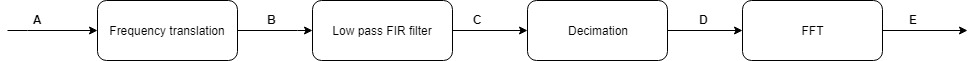
\includegraphics[scale=0.4]{zoom_fft_diagram}
	\decoRule
	\caption{A block diagram showing the zoom FFT algorithm. This figure was created with Draw.io.}
	\label{fig:zoom_fft_diagram}
\end{figure}

The computational reduction for a Zoom FFT is shown in Figure \ref{fig:zoom_fft_complexity_reduction}.  However, it is important to note that a stronger filter is required for higher decimation factors, $D$.  This means there is a trade-off between FFT computational load and filter computational load.  A zoom FFT is just the name of a method of frequency transformation where the data is decimated before applying the FFT algorithm.  The computational savings occur when a well-designed lowpass filter does not negate the workload reduction caused by the FFT.  Essentially, this is a much more flexible FFT where different aspects can be modified to optimize for the application.  In this case, the Zoom FFT can provide a much higher resolution frequency analysis because the frequencies of interest are much smaller than the sampling rate.


\begin{figure}
	\centering
	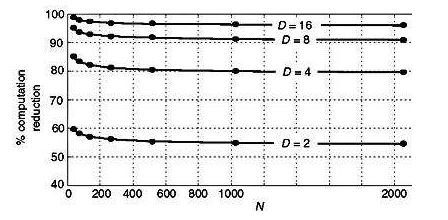
\includegraphics[scale=0.8]{zoom_fft_complexity_reduction}
	\decoRule
	\caption{A diagram showing the percent computational workload reduction of a $\frac{N}{D}$-point Zoom FFT relative to a standard $n$-points FFT \cite{embedded_zoom_fft}.}
	\label{fig:zoom_fft_complexity_reduction}
\end{figure}



\subsubsection{Frequency translation}
Shifting data in the frequency domain is a common technique used in AM radio signals.  Audio frequencies are typically mixed with a high frequency carrier that, according to the Nyquist criteria, would require an extremely high sample rate to capture the signal.

If $\omega$ is the rotor frequency, multiplying the time domain signal by $\cos{(-\omega t)}$ is the same as convolving the data in the frequency domain.  Since the frequency spectra for $\cos{(-\omega t)}$ is symmetric across the y-axis, the time-domain must be multiplied by an imaginary wave.

The equation for the frequency-shifted time-domain data is:
\begin{equation} \label{eq:frequency_translation}
	Y = X e^{-i (\omega t)}
\end{equation}

where $Y$ is the shifted data, $X$ is the original data, $\omega$ is the rotor frequency, and $t$ is the time.  Based on Equation \ref{eq:frequency_translation}, the real and imaginary parts of the shifted signal are shown below \cite{zoom_fft_ref}:
\begin{align}
	Y_{real} = X \cos{(\omega t)} \\
	Y_{imaginary} = -X \sin{(\omega t)} \label{eq:freq_trans_im}
\end{align}

An example of frequency translation is shown in Figure \ref{fig:MATLAB_freq_translation_ex}.  The blue signal is the frequency-shifted signal, which has a higher frequency at 2 times the original signal frequency.  In order to remove the extra component at 10 Hz, the digital filter (shown with a dotted blue line) must be applied to the shifted signal.

\begin{figure}
	\centering
	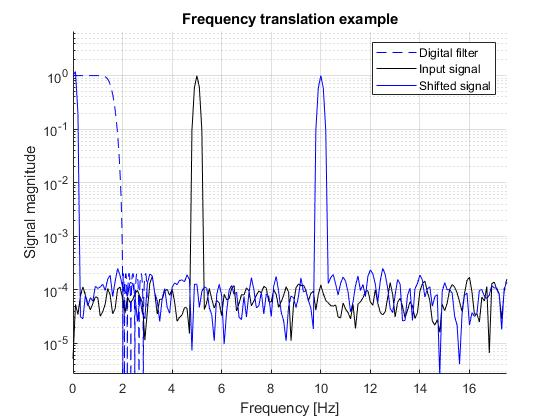
\includegraphics[scale=0.7]{MATLAB_freq_translation_ex}
	\decoRule
	\caption{This figure shows an example of frequency translation.  The black signal is the frequency spectrum of some input signal that has a strong component at 5 Hz.  The blue signal shows the frequency shifted spectrum that results from multiplying the input signal by a reference signal with a frequency of 5 Hz (as shown in Equation \ref{eq:freq_trans_im}.  The dotted blue line shows the digital filter response.  This figure was generated with MATLAB.}
	\label{fig:MATLAB_freq_translation_ex}
\end{figure}

\subsubsection{Decimation/downsampling}
Decimation is the process of reducing the sample rate of a signal.  Before the data is downsampled, the high frequency components are reduced with a lowpass filter. This filter is also called an anti-aliasing filter because it prevents high frequency data from being misinterpreted at a different sample rate.  Equation \ref{eq:decimation} shows the equation used for calculating the output of a FIR decimator, where $x$ is the input data, $h$ is the impulse response, $K$ is the length, and $D$ is the decimation factor\cite{decimation_ref}.
\begin{equation} \label{eq:decimation}
	y[n] = \sum_{k=0}^{K-1} x[nD-k] \cdot h[k]
\end{equation}

Figure \ref{fig:MATLAB_freq_translation_ex} shows a visual representation of the decimation process and anti-aliasing filter.  The shifted signal (blue) contains important frequency information in the range 0 - 2 Hz.  Any higher frequencies have been significantly attenuated by the digital filter (dotted blue line).  This means the blue data can be decimated to a new sampling rate of 4 Hz, without any aliasing effects (because the digital filter ensures there are no strong components above 2 Hz).



\subsubsection{An optimized Zoom FFT implementation}

Table \ref{t:zoom_fft_parameters} shows the parameters for the Zoom FFT.  These values have been strategically picked to make the optimization process easier.  In general, some nice optimizations can be achieved if the number of filter coefficients ($N_b+1$) is an integer multiple of the sampling rate ($F_s$).

\begin{table}[]
\centering
\caption{Zoom FFT parameters}
\label{t:zoom_fft_parameters}
\vspace*{0.2in}
\begin{tabular}{|c|c|c|}
\rowcolor[HTML]{EFEFEF} 
\hline
\textbf{Variable} & \textbf{Value} & \textbf{Description} \\ \hline
$F_{min}$ & 2 Hz & The minimum frequency for the Zoom FFT calculation\\ \hline
$F_s$ & 128 Hz & The original sampling rate\\ \hline
$F_r$ & 4 Hz & The frequency range of the Zoom FFT\\ \hline
$N_{fft}$ & 128 & FFT length (buffer length used in the FFT calculation)\\ \hline
$N_b$ & 255 & FIR filter order \\ \hline
$D$ & $\frac{F_s}{2 F_r}=16$ & Decimation rate \\ \hline
\end{tabular}
\end{table}

In Table \ref{t:zoom_fft_parameters}, the FFT length is the number of samples in the buffer used as the input to the FFT. An FFT length of 1024 means that 1024 samples are used as an input to the FFT algorithm.  The FIR filter order is 255, which is high because it needs to strongly attenuate higher frequencies with a narrow pass band.  Despite having an extremely large order, the FIR filter is simple and computationally inexpensive to implement (this will be shown later in this section).  An order of $N_b=255$ means the filter order will have 256 ($N_B+1$) coefficients.  $F_{min}$ and $F_r$ define the frequency range that the Zoom FFT is targeting.  More specifically, the Zoom FFT will calculate the frequency spectrum of the input signal only from $F_{min}$ to $F_{r}$.  The filter design is highly motivated by the frequency range because it needs to attenuate the original signal sufficiently (to prevent aliasing at the decimation step) at the edge of the frequency range.

The reference signal for the Zoom FFT is created at the minimum frequency, $F_{min}$ shown in Table \ref{t:zoom_fft_parameters} and is shown in Equation \ref{eq:zoom_ref_sig}.
\begin{equation} \label{eq:zoom_ref_sig}
	y_{ref} = \sin{(F_{min} \cdot 2\pi \cdot time)}
\end{equation}

Note that there are only 64 unique values in a reference signal with the specified $F_{min}$.  This means that all of these values can be precomputed at initialization and stored in memory.  This removes the $\sin{()}$ operations from the real-time calculations, which reduces the computational time, since trig functions are one of the slowest floating-point operations (they are typically about 15X slower than a floating-point addition operation) \cite{flops_performance}.

One of the benefits for using a finite impulse response (FIR) filter is that there are no recursive calculations.  This produces a very important property of FIR filters, which is that not all the outputs need to be calculated.  Assuming there are ($N_b+1$) filter coefficients, a random window of ($N_b+1$) samples can be properly filtered at any time during operation.  If we are decimating the input signal, this means we do not have to calculate the filter outputs for samples that are removed due to the decimation step.

The down-sampled data, $y_{ds}$, can be calculated as follows ($\odot$ is the element-wise multiplication operator):
\begin{equation} \label{eq:zoom_y_ds}
	y_{ds} = \vec{y}^T \cdot \left( \vec{y}_{ref} \odot 2\vec{b} \right)
\end{equation}

In Equation \ref{eq:zoom_y_ds},  $y_{ds}$ is the value at the decimated sampling rate.  $\vec{y}$ is a sliding buffer of the original input data, which is a vector of ($N_b+1$) values.  $\vec{y}_{ref}$ is the vector of the reference signal values, which also has a length of ($N_b+1$).  $\vec{b}$ is the vector of FIR filter coefficients.  The factor of 2 in this equation is a result of the derivation of the frequency-shift process.  Equation \ref{eq:zoom_y_ds} is calculated at the decimated sampling rate ($F_{sD}$), which is shown in Equation \ref{eq:zoom_dec_Fs}.
\begin{equation} \label{eq:zoom_dec_Fs}
	F_{sD} = \frac{F_s}{D}
\end{equation}

Equation \ref{eq:zoom_y_ds} can also be used with larger filter orders.  Effectively, this means that the filtering and decimation part of the Zoom FFT can be performed with just a single dot product and an element-wise vector multiplication.  Using the values in Table \ref{t:zoom_fft_parameters}, the following steps can be followed to create a Zoom FFT algorithm:
\begin{enumerate}
	\item Precompute the unique values of the reference signal during initialization.
	\item Design a FIR filter with an appropriate cutoff frequency and filter order.  The cutoff frequency ($F_{cutoff}$) is equal to the frequency range ($F_r$) of the Zoom FFT.  The coefficients of this filter are stored in $\vec{b}$.
	\item Generate a sliding buffer of data with a window size of ($N_b+1$) and an overlap of ($N_b+1 - \frac{F_s}{D}$), which is stored in $\vec{y}$.
	\item Perform the calculation shown in Equation \ref{eq:zoom_y_ds}.
	\item Calculate the FFT of the newly decimated data.
\end{enumerate}

Figure \ref{fig:MATLAB_zoom_fft_ex} shows the results of a MATLAB simulation using the Zoom FFT to calculate the frequency spectrum.  In this simulation, the standard FFT uses an FFT length of 2048, while the Zoom FFT only has a length of $N_{fft}=128$.  This is a significant reduction in computation for the same frequency resolution in the target Zoom FFT range.  Both a standard FFT and a Zoom FFT use the same FFT algorithm, so the difference in performance comes from the lower sampling rate, and therefore smaller frequency range.

\begin{figure}
	\centering
	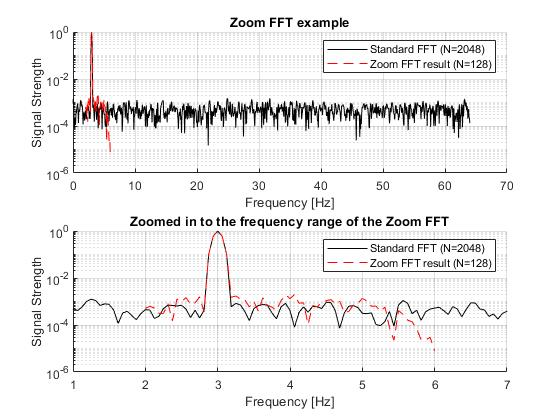
\includegraphics[scale=0.7]{MATLAB_zoom_fft_ex}
	\decoRule
	\caption{This figure shows the results of a Zoom FFT using the parameters listed in Table \ref{t:zoom_fft_parameters}.  The top plot shows the frequency spectrum from a standard FFT (black) and a Zoom FFT (red).  The bottom plot shows the same data as the top plot, but zoomed into a narrow frequency range. The standard FFT has a length of 2048, while the Zoom FFT has a length of 128.  This figure was created with MATLAB.}
	\label{fig:MATLAB_zoom_fft_ex}
\end{figure}

\subsubsection{Estimating processor performance}
Comparing the computational time of different algorithms is difficult because the dominant factor is usually memory access, rather than actual floating-point operations \cite{wiki_fft}.  Evaluating the computational cost due to memory access patterns in complicated, so this analysis will only consider the computational cost of the floating-point operations (FLOPs).  To minimize the cost from memory access patterns, the algorithms will be vectorized and converted to matrix form.  Most processors have highly optimized matrix operation functions, which should hopefully make arithmetic the dominant factor when determining the computational cost.

For this analysis, a STM32 processor is used as the baseline for estimating cycle counts because it is the unit used to prototype the LifeLine data acquisition device that collects experimental acceleration data from the turbine.  The STM32 has its own single precision register set to handle floating-point operations with hardware (rather than using compiled C libraries to perform the floating-point operations in many complex steps).  The floating-point unit (FPU) in the STM32 offers arithmetic instructions for the operations listed in \todo{Table XXX} \cite{stm32_floating_point}.

Many FPUs (like the one in \todo{Table XXX}), have multiply/accumulate arithmetic instructions, which means they can perform a multiplication and addition all in one step.  Additionally, division operations are much more expensive than multiplication operations and should be avoided as much as possible when designing algorithms.

\begin{table}[]
\centering
\caption{Cycle counts for a STM32 floating-point processor}
\label{t:stm32_cycles}
\vspace*{0.2in}
\begin{tabular}{|c|c|}
\rowcolor[HTML]{EFEFEF} 
\hline
\textbf{Operation} & \textbf{Cycles} \\ \hline
Absolute value & 1 \\ \hline
Negate of a float & 1 \\ \hline
Addition/subtraction & 1 \\ \hline
Multiply & 3 \\ \hline
Multiply and accumulate/subtract & 3 \\ \hline
Divide & 14 \\ \hline
Square Root & 14 \\ \hline
Exponential & 20* \\ \hline
\end{tabular}
\end{table}



\subsection{Goertzel Algorithm}
The Goertzel algorithm is a method for calculating individual bins of a discrete Fourier transform (DFT) without calculating all of the bins.  Since imbalance detection depends on the strength of the rotor frequency, this algorithm produces the particular rotor frequency bin value without calculating the entire DFT.  Fundamentally, this algorithm operates similarly to the Zoom FFT previously described, and is often called a Goertzel filter because the algorithm takes the form of a digital filter.  This algorithm applies 2 stages of filtering, where the first stage is an infinite impulse response (IIR) filter, and the second stage is a finite impulse response (FIR) filter.

For the first stage of the Goertzel algorithm, a 2nd order IIR filter is applied to $x$:
\begin{equation}
	s[n] = x[n] + 2 \cos{(\omega_0)}s[n-1] - s[n-2] \\
\end{equation}

This IIR filter follows a Direct Form II structure, where 2 state variables are required for a 2nd order filter.  $\omega_0$ is defined as the normalized frequency to be analyzed.

The second stage of the algorithm is a FIR filter, which is known for its linear phase, and lack of feedback.  This means that the filter output does not depends on any previous outputs.
\begin{equation} \label{eq:goertzel_output}
	y[n] = s[n] - e^{-j\omega_0}s[n-1]
\end{equation}

Equation \ref{eq:goertzel_output} shows the output of the Goertzel equation, $y[n]$.

There is an optimized version of the Goertzel algorithm that is even faster than the general form, but it produces squared magnitude components at each frequency instead of real/imaginary pairs \cite{embedded_goertzel}.  The phase of the frequency component is not used in the imbalance detection algorithm, so the optimized Goertzel algorithm is well suited for this application.  One of the benefits of the Goertzel algorithm is the buffer lengths do not need to be a power of 2.  An overview of the algorithm in a block diagram form is shown in Figure \ref{fig:goertzel_diagram_ti}.

The Goertzel algorithm is simulated with MATLAB and the results are shown in Figure \ref{fig:MATLAB_goertzel_algorithm_ex}.  The Goertzel algorithm calculates individual frequency components of the DFT, which are identical to the values calculated with a standard FFT algorithm.

\begin{figure}
	\centering
	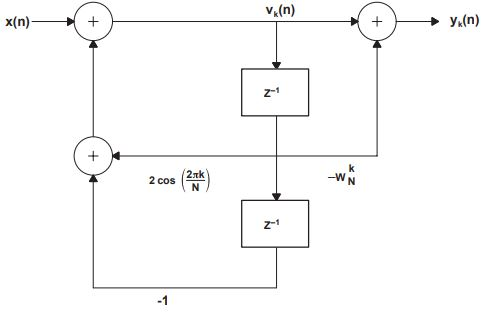
\includegraphics[scale=0.7]{goertzel_diagram_ti}
	\decoRule
	\caption{The direct-form realization of the Goertzel Algorithm\cite{TI_goertzel}.}
	\label{fig:goertzel_diagram_ti}
\end{figure}

\begin{figure}
	\centering
	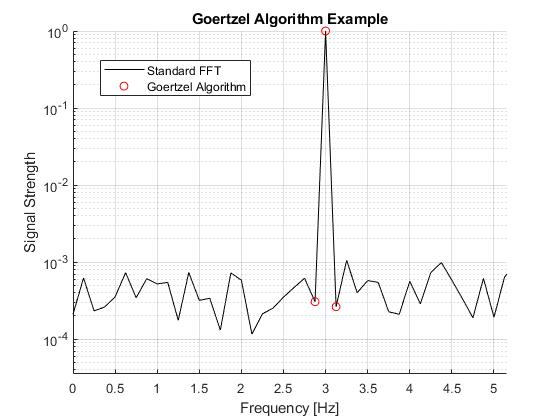
\includegraphics[scale=0.7]{MATLAB_goertzel_algorithm_ex}
	\decoRule
	\caption{This figure shows the frequency spectrum calculated with a standard FFT (black) and a few points calculated with the Goertzel algorithm (red).  This figure was created in MATLAB.}
	\label{fig:MATLAB_goertzel_algorithm_ex}
\end{figure}

\chapter{Imbalance Detection Algorithm} % Chapter title
\label{ch_detection_algorithm}

%----------------------------------------------------------------------------------------
%	Overview
%----------------------------------------------------------------------------------------
\section{Overview}
A rotor imbalance can causes problems and failures with the turbine, so it is important to detect the ``state" of the turbine using some measured input.  Turbine dynamics are complicated, vary between different systems and can be dependent on many variables.  An effective way to develop a model that is optimized for each different turbine is to use machine learning (ML).  Machine learning is the study of algorithms that build mathematical models to perform specific tasks without explicit instructions.

\subsection{Machine learning background}
The 2 main types of machine learning algorithms are supervised and unsupervised learning.  Supervised algorithms assume that each data set is assigned an output, while unsupervised algorithms take a data set of only inputs and attempt to create groups and classes from the input data.  For this application, each measurement data set from the turbine will be manually labeled as ``good" or ``bad" (or as ``balanced"/``unbalanced"), which is a type of supervised learning.

Machine learning algorithms also fall into the ``regression" or ``classification" categories.  Regression algorithms are used if the output is a continuous function, while classification algorithms are used if the output falls into distinct classes.  The output for the turbine detection algorithm is the state of the turbine (balanced/imbalanced), which is a discrete classification.

Knowing that the ML algorithm must be a classification, supervised model, the specific algorithm choice can be narrowed down.  Some of the common algorithms are logistic regression (this can be used as a classification algorithm even though it is called ``regression"), k-nearest neighbor, and neural networks.  This paper will analyze each of these models and apply them to the experimental turbine data.

\section{The training data}
Typically, it is common for machine learning algorithms to split the data into test and training sub groups.  This allows the accuracy of the models to be trained and evaluated on different data sets.  The input data for the turbine is a 256-point frequency spectrum of the acceleration data at the top of the tower.  This data is obtained using the LifeLine system, which includes an accelerometer and a STM32 microprocessor.  This device is placed at the top of the tower and powered directly from the turbine.  Ideally, this device would significantly drop the clock rate of the processor or swap out the processor for an extremely low-power one.  This would allow the device to be wireless and have a reasonable operation time for each battery charge.  Figure \ref{fig:LL_spectrogram} shows a spectrogram of the measured acceleration data from the LifeLine device.  A spectrogram is a way to visualize frequency data over time in a 2-dimensional figure, where the magnitudes of each frequency component are represented by a different color.  The spectrogram shows that there is a strong frequency component at about 2.4 Hz (the rotor frequency) that is constant throughout most of the operation.

\begin{figure}
	\centering
	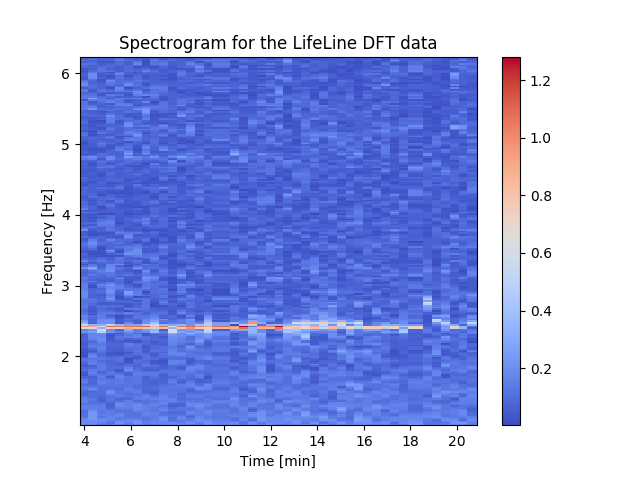
\includegraphics[scale=0.8]{LL_spectrogram}
	\decoRule
	\caption{This figure shows the spectrogram of the tower accelerations.  This figure was created with Python.}
	\label{fig:LL_spectrogram}
\end{figure}

Currently, only a single set of about 100 training examples exists.  The data can be separated into 2 classes; however, there is no information about which is the \textit{balanced} and \textit{imbalanced} classes.  To properly train the machine learning models, more data is required.  Despite the lack of available data, this paper will discuss the methods and implementations of each algorithm using the limited data set.


\section{K-Nearest Neighbor algorithm}
\section{About the algorithm}
The k-nearest neighbor (KNN) algorithm is one of the simplest models, but can be the most accurate and powerful when dealing with fairly small data sets.  This model essentially ``memorizes" the training data and plots the points in $n$-dimensional space.  The classification of a new point is calculated based on the distances between the new point and the training points.  For example, Figure \ref{fig:knn_visualization} shows a visualization of the classification process for a 2-class system.  Since this algorithm uses all of the training data in memory, it becomes very slow with many inputs, and many training data sets.  The example in Figure \ref{fig:knn_visualization} is a 2-dimensional problem (only 2 inputs) with only a few data points, so the KNN algorithm works very well.


\begin{figure}
	\centering
	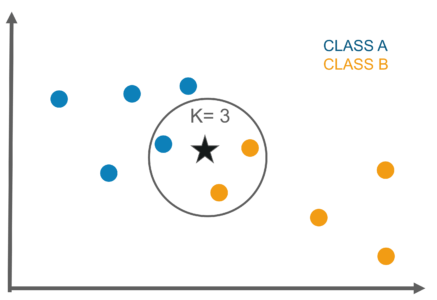
\includegraphics[scale=0.4]{knn_visualization}
	\decoRule
	\caption{A visualization of the KNN algorithm \cite{knn_python}.  The training data for a 2-class problem with 2 inputs is shown as blue and orange dots.  For $K=3$, a circle is drawn around the new point (star) until 3 training data points fall within the circle.  The classification of the new point is then determined by the majority of the points inside the circle.  In this case, there are more \textit{Class B} points than \textit{Class A} points, so the new point (star) will be classified as \textit{Class B}.}
	\label{fig:knn_visualization}
\end{figure}

The K-NN algorithm uses a "majority voting" method where the Euclidian distance between all the training data points and the test data is calculated.  This model assumes there is a relatively equal amount of balanced rotor experimental data and imbalanced experimental rotor data, which means the sample weighting can be uniform.  If there is a much higher frequency class (for example, much more balanced experimental data), this class will tend to dominate the calculations regardless of the actual class of the test data.

The number of neighbors, $k$, is chosen to be 3 for this algorithm (using trial and error).  A larger value of $k$ will reduce the classification noise, but the boundaries are much more general and not as tuned to the training data.  A lower value of $k$ will match the model very closely to the training data, but may add noise into the classification process.

The Euclidean distance is simply the distance between the data points.  This equation is shown below:

\begin{equation}
	d = \sqrt{\sum{\left(x_{i,a}-x_{j,a}\right)^2}}
\end{equation}

\subsection{Choosing the data}
The KNN algorithm works well on small data sets, so the DFT data should be pre-processed and cut down to a smaller, 2-dimensional data set.  Based on a simplified dynamic model of the turbine tower, a rotor imbalance will cause a high frequency excitation at the rotor frequency.  Using the maximum frequency component of the experimental DFT data and the corresponding frequency is a good way to capture enough information about the tower, while also reducing the data set from 256 input points to only 2 input points.

Figure \ref{fig:single_dft} shows the frequency spectrum from a single DFT calculation.  To convert this data into 2-dimensional data for the KNN algorithm, the peak value and corresponding frequency are extracted from this data.  For example, Figure \ref{fig:single_dft} would produce a 2-dimensional data set as shown in Equation \ref{eq:2d_data}.
\begin{equation} \label{eq:2d_data}
	[x_1, x_2, y] = [frequency, amplitude, class] = [2.3, 1.0, Class A]
\end{equation}

\begin{figure}
	\centering
	\includegraphics[scale=0.4]{single_dft}
	\decoRule
	\caption{This figure shows a single DFT result (a single column from Figure \ref{fig:LL_spectrogram}).  This figure was created with Python.}
	\label{fig:single_dft}
\end{figure}

By converting the entire data set for all training examples into 2-dimensional data, the data in Figure \ref{fig:LL_spectrogram} can be represented as the data in Figure \ref{fig:max_balanced_freq_mag}.

\begin{figure}
	\centering
	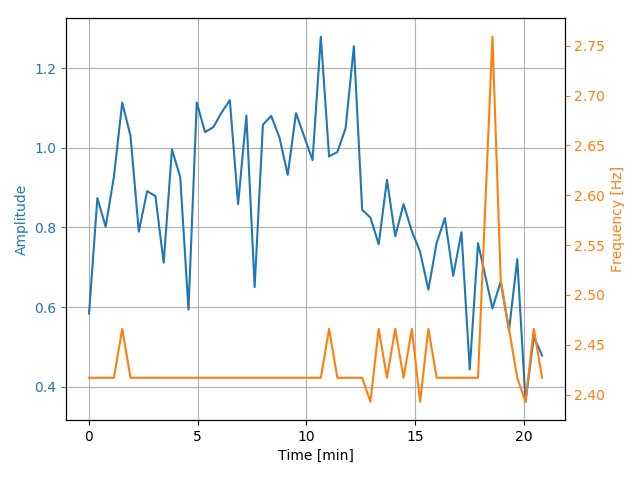
\includegraphics[scale=0.8]{max_balanced_freq_mag}
	\decoRule
	\caption{This figure shows a the 2-dimensional data used as an input to the KNN classification algorithm.  This figure was created with Python.}
	\label{fig:max_balanced_freq_mag}
\end{figure}


\subsection{Algorithm Results}
To apply the algorithm, the data is converted into short lists containing a maximum amplitude, a corresponding frequency value, and the known class (Equation \ref{eq:2d_data}). For this test, there are 55 experimental DFT results for \textit{Class A} and 55 experimental DFT results for \textit{Class B}. 

Training the KNN model is extremely fast and only involves storing all of the training data in memory.  When the algorithm is applied to new test examples, the results can be visualized in a confusion matrix \cite{confusion_matrix} as shown in Equation \ref{eq:knn_confusion_matrix}.  A confusion matrix is a common tool used to describe the performance of a classification algorithm.  This is an $n$ by $n$ matrix (where $n$ is the number of classes) that essentially shows the amount of correct and incorrect guesses for each class.  Table \ref{t:confusion_matrix_ex} shows a labeled version of the confusion matrix shown in Equation \ref{eq:knn_confusion_matrix}.

\begin{equation} \label{eq:knn_confusion_matrix}
C_{confusion} = 
\begin{bmatrix}
	12 & 1 \\
	3 & 6
\end{bmatrix}
\end{equation}

\begin{table}[]
\centering
\caption{An example of the terminology for the confusion matrix in Equation \ref{eq:knn_confusion_matrix}. \textit{Class A} and \textit{Class B} represent the different classes of data.  These can be related to a \textit{balanced} and \textit{imbalanced} rotor with proper data set labels.}
\label{t:confusion_matrix_ex}
\vspace*{0.2in}
\begin{tabular}{lllll}
\cline{2-3}
\multicolumn{1}{l|}{}                      & \multicolumn{1}{l|}{\textbf{Predicted Class A}} & \multicolumn{1}{l|}{\textbf{Predicted Class B}} &  &  \\ \cline{1-3}
\multicolumn{1}{|l|}{\textbf{Actual Class A}}  & \multicolumn{1}{l|}{12}                     & \multicolumn{1}{l|}{1}                       &  &  \\ \cline{1-3}
\multicolumn{1}{|l|}{\textbf{Actual Class B}} & \multicolumn{1}{l|}{3}                      & \multicolumn{1}{l|}{6}                       &  &  \\ \cline{1-3}
                                           &                                             &                                              &  & 
\end{tabular}
\end{table}


\begin{figure}
	\centering
	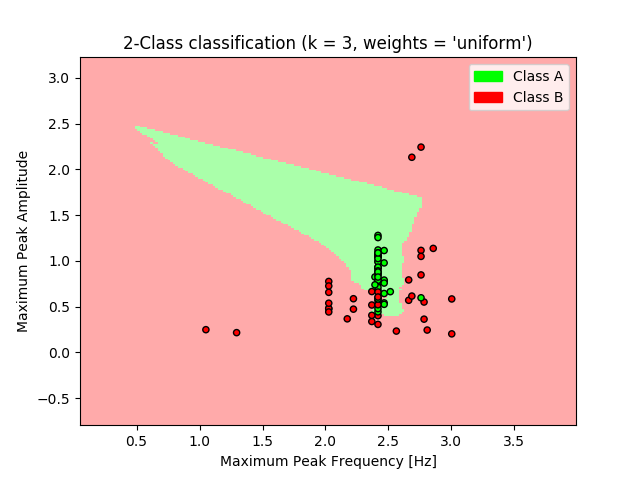
\includegraphics[scale=0.8]{knn_decision_boundary_k_3}
	\decoRule
	\caption{This figure shows the classification boundary for the KNN algorithm with $K=3$ for all of the training data.  This figure was created with Python.}
	\label{fig:knn_decision_boundary_k_3}
\end{figure}

A nice way to visualize the results of the classification algorithm with 2-dimensional inputs is to create a decision boundary plot.  A decision boundary is the area in space where the algorithm switches to a different classification.  Figure \ref{fig:knn_decision_boundary_k_3} shows the classification boundary for the KNN algorithm with $K=3$.

Initially, the balanced and imbalanced classes were expected to be easily distinguishable from each other.  Despite not having accurate labels of the experimental data, the imbalanced rotor data was expected to have much higher amplitudes at the rotor frequency; however, from Figure \ref{fig:knn_decision_boundary_k_3}, there isn't a significant difference between the amplitudes of the 2 data classes.

One observation that can be made from the data shown in Figure \ref{fig:knn_decision_boundary_k_3} is that the Class A data seems to have more frequency stability.  The Class A data has a constant frequency of about 2.5 Hz, while the Class B data has varying frequencies.  There is not enough data to make any hard conclusions, but this variance could be caused by either wind speed fluctuations or an actual property of the imbalance.  It is possible that an imbalance in the rotor could cause more variations in rotor speed, despite not having significant amplitude differences.  However, until the data can be accurately labeled, or more experimental data is collected, these classes should remain Class A and Class B to avoid any incorrect assumptions about the rotor imbalance.

\section{Logistic Regression}
\subsection{About the algorithm}
Logistic regression (LR) is a modified version of linear regression that is adapted for classification problems.  Logistic regression minimizes the squared error of a linear combination of the input parameters when passed through a sigmoid function.  To fully understand logistic regression, a brief background of linear regression is required. 

Linear regression is the process of minimizing the least squares cost of a data set with a linear function.  This is a commonly utilized method in curve fitting, but can also be applied to very high order systems.  Mathematically, this means minimizing the cost function shown in Equation \ref{eq:linear_regression_cost_fun}.  The hypothesis is the linear curve fit shown in Equation \ref{eq:linear_regression_hypothesis}.
\begin{align}
	J\left(\vec{\theta}\right) &= \frac{1}{2m} \sum_{i=1}^{m}{\left(h_{\theta}(x_i) - y_i\right)^2} \label{eq:linear_regression_cost_fun} \\
	h_{\theta}(x) &= \mat{x} \cdot \vec{\theta}^T \label{eq:linear_regression_hypothesis} \\
	\vec{\theta} &= [\theta_0, \theta_1, \theta_2, \theta_3, \hdots, \theta_n]
\end{align}

$n$ is the number of parameters (or features) in the input, $\mat{x}$.  $m$ is the number of training examples, which means $\mat{x}$ is of size $[m, n]$ and $\vec{\theta}$ is a vector with $n$ elements.

In order to apply linear regression to classification problems, the sigmoid function is applied to the linear regression hypothesis ($h_{\theta}$).  The sigmoid function is defined in Equation \ref{eq:sigmoid_function} and is visually shown in Figure \ref{fig:sigmoid_plot}.  The sigmoid function is designed to map an input to a value between 0 and 1, which represents the probability that the input is of a certain class.  This sigmoid function is what enables logistic regression to calculate binary outputs.
\begin{equation} \label{eq:sigmoid_function}
	g(z) = \frac{1}{1+e^{-z}}
\end{equation}

\begin{figure}
	\centering
	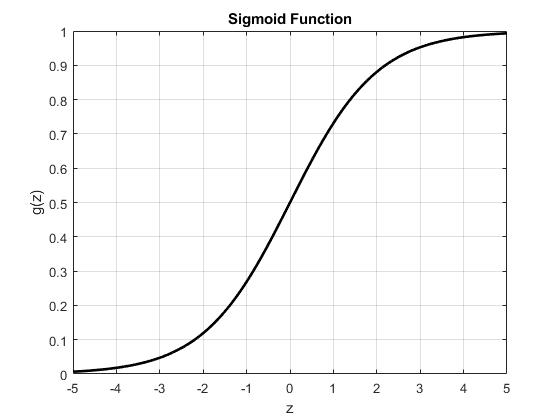
\includegraphics[scale=0.6]{sigmoid_plot}
	\decoRule
	\caption{This figure shows the sigmoid function plot.  This figure was created with MATLAB.}
	\label{fig:sigmoid_plot}
\end{figure}

This new hypothesis function (Equation \ref{eq:logistic_regression_hypothesis}) produces a new cost function, shown in Equation \ref{eq:logistic_regression_cost}.
\begin{align}
	J(\theta) &= \frac{1}{m} \sum_{i=1}^{m}{\left[y_i \ln({h_{\theta}(x_i))} + (1-y_i) \ln{(1-h_{\theta}}) \right]}  \label{eq:logistic_regression_cost} \\
	h_{\theta} &= g(\mat{x} \cdot \vec{\theta}^T) = \frac{1}{1+e^{-(\mat{x} \cdot \vec{\theta}^T)}} \label{eq:logistic_regression_hypothesis}
\end{align}

The goal of logistic regression is to create a model that best fits the experimental training data by optimizing the parameters $\vec{\theta}$ to minimize the cost function, $J(\theta)$.  To do this, the gradient descent method is used \cite{gradient_descent}.  To  perform gradient descent, both the cost function and the gradient function of $\vec{\theta}$ are required.  The gradient can be numerically calculated using the finite difference method \cite{finite_difference_method}; however, this is much more computationally intensive than directly calculating the gradient analytically.  The derivative of the sigmoid function is shown in Equation \ref{eq:sigmoid_derivative}.  This produces a simple equation for the gradient of the cost function, which is shown in Equation \ref{eq:logistic_regression_gradient}.
\begin{align}
	g\prime(z) &= g(z) (1-g(z)) \label{eq:sigmoid_derivative} \\
	\frac{\partial J(\theta)}{\partial \theta_j} &= \frac{1}{m} \sum_{i=1}^{m}{\left(h_{\theta}(x_i) - y(i)\right) x_{j,i}} \label{eq:logistic_regression_gradient}
\end{align}

$h_{\theta}$ is defined in Equation \ref{eq:logistic_regression_hypothesis} and $g(z)$ is defined in Equation \ref{eq:logistic_regression_cost}.  In other words, Equation \ref{eq:logistic_regression_gradient} represents an average of $(h-y)x$ for every training example and calculated with respect to each $\theta$ parameter ($j$ is the number of parameters in the model).

\subsection{Training the model}
To train the model, the cost function is minimized using a version of the gradient descent optimization process.  This iterates through various values of $\theta$ that are calculated using the gradient of the cost function.  Figure \ref{fig:logistic_regression_2_feature_cost} shows the cost function over the iteration (training) process.  When the cost function has converged to a minimum, the model training is complete and the model is ready to be validated on the test data.

\begin{figure}
	\centering
	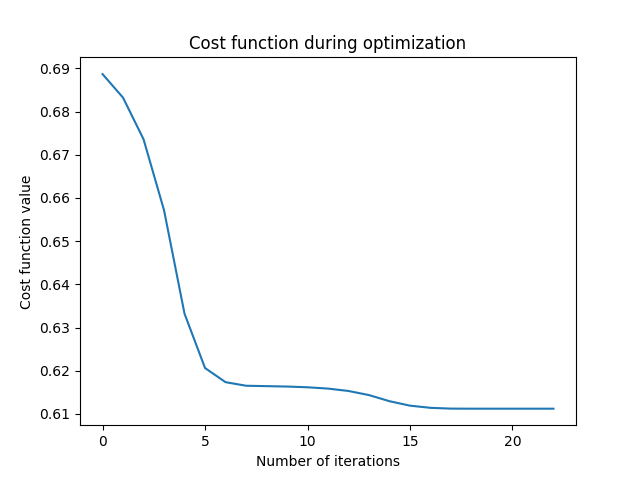
\includegraphics[scale=0.8]{logistic_regression_2_feature_cost}
	\decoRule
	\caption{This figure shows the cost function during the training process.  This model uses 2 features, so the model is trying to optimize $\vec{\theta} = [\theta_0, \theta_1, \theta_2]$ (3 parameters because there is a hidden bias unit).  This figure was created with Python.}
	\label{fig:logistic_regression_2_feature_cost}
\end{figure}

\subsection{Applying the model}
Minimizing the cost function results is a trained model that produces the decision boundary shown in Figure \ref{fig:logistic_regression_decision_boundary}.  This model has a pretty poor accuracy of about 67\% on the test data.

\begin{figure}
	\centering
	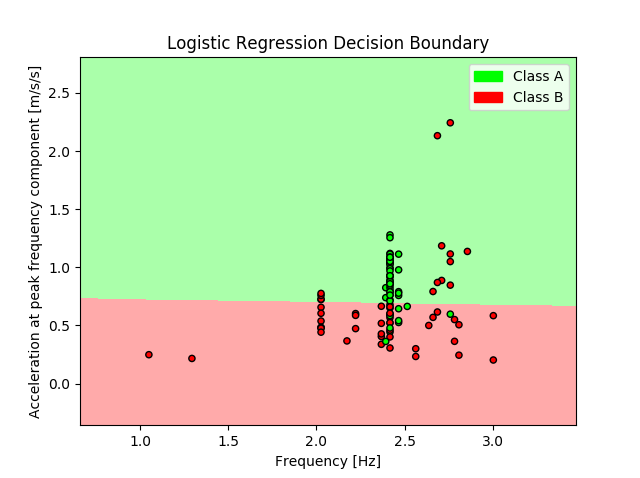
\includegraphics[scale=0.8]{logistic_regression_decision_boundary}
	\decoRule
	\caption{This figure shows the decision boundary from the logistic regression model.  This is a linear model using 2 input parameters and a binary output class.  This model has an accuracy of about 67\% when using the test data set.  This figure was created with Python.}
	\label{fig:logistic_regression_decision_boundary}
\end{figure}

To improve this model, the 2 input parameters can be expanded to create a higher order models.  For example, the 2 input features for a linear logistic regression model are shown in Equation \ref{eq:lr_order1}.  To achieve higher order models, the input parameters can be expanded to included the terms for the higher order polynomials.  This will allow the regression to fit parameters to each of the new inputs.  Equation \ref{eq:lr_order2} represents the input variables expanded for a 2nd order model and Equation \ref{eq:lr_order3} represents the input variables expanded for a 3rd order model.  Figure \ref{fig:logistic_regression_order2_decision_boundary} shows the decision boundary for a 2nd order model and Figure \ref{fig:logistic_regression_order3_decision_boundary} shows the decision boundary for a 3rd order model.
\begin{align}
	[x_1, x_2]  \label{eq:lr_order1} \\
	[x_1, x_2, x_1^2, x_1 x_2, x_2^2] \label{eq:lr_order2} \\
	[x_1, x_2, x_1^3, x_1^2 x_2, x_1 x_2^2, x_2^2] \label{eq:lr_order3}
\end{align}

\begin{figure}
	\centering
	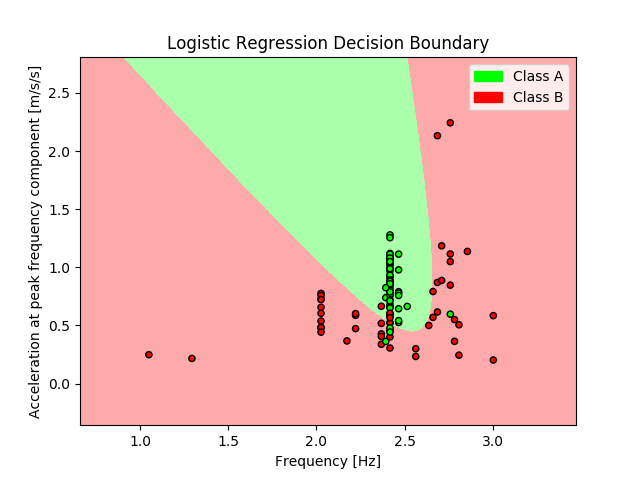
\includegraphics[scale=0.8]{logistic_regression_order2_decision_boundary}
	\decoRule
	\caption{This figure shows the decision boundary from the logistic regression model.  This is a 2nd order model using 2 input parameters and a binary output class.  This model has an accuracy of about 85\% when using the test data set.  This figure was created with Python.}
	\label{fig:logistic_regression_order2_decision_boundary}
\end{figure}

\begin{figure}
	\centering
	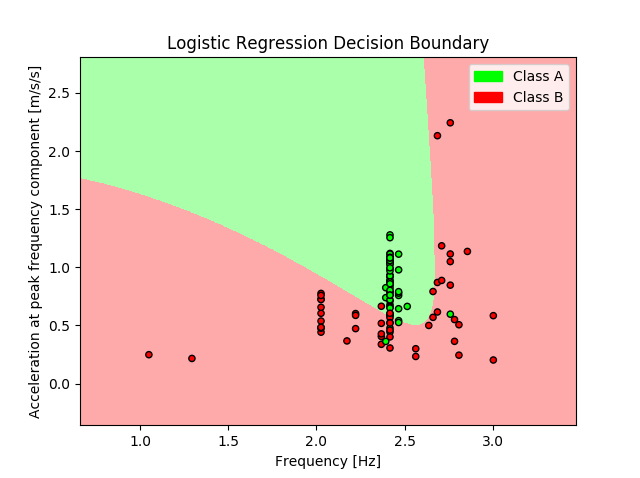
\includegraphics[scale=0.8]{logistic_regression_order3_decision_boundary}
	\decoRule
	\caption{This figure shows the decision boundary from the logistic regression model.  This is a 3rd order model using 2 input parameters and a binary output class.  This model has an accuracy of about 85\% when using the test data set.  This figure was created with Python.}
	\label{fig:logistic_regression_order3_decision_boundary}
\end{figure}

In fact, the order can keep getting increased until the model fits the training data perfectly.  This is called over-fitting and is a problem with higher order machine learning models.  Figure \ref{fig:logistic_regression_order10_decision_boundary} shows an example of a 10th order model that has some over-fitting problems.  It is unlikely that the small region separating the Class A sections (at about 2.5 Hz and 1.5 m/s/s) belongs to Class B.  In order to solve the problem of over-fitting, a regularization term can be added to the cost function equation.  This regularization term, $\lambda$, effectively reduces the impact that the optimization parameters have on the cost calculation, which keeps the optimized parameters small.  This reduces the ``strength" of the regression model and can help eliminate over-fitting problems.  Equation \ref{eq:logistic_regression_cost_reg} shows the new logistic regression cost function with a regularization term applied.  The new gradient function can be derived with the regularization term, as shown in Equation \ref{eq:logistic_regression_gradient_reg}.

\begin{figure}
	\centering
	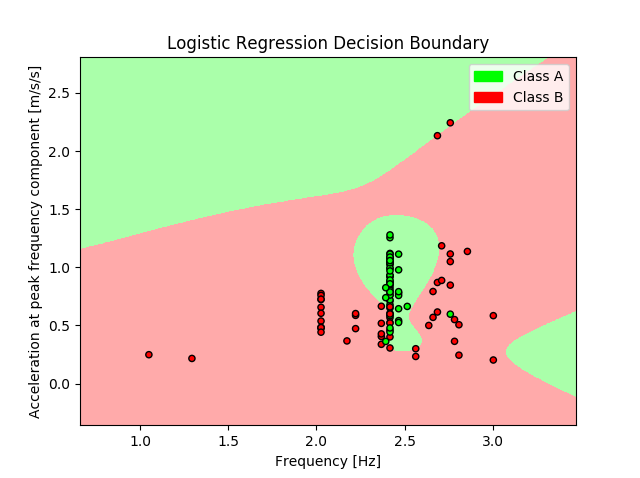
\includegraphics[scale=0.8]{logistic_regression_order10_decision_boundary}
	\decoRule
	\caption{This figure shows the decision boundary from the logistic regression model.  This is a 10th order model using 2 input parameters and a binary output class, and has an over-fitting problem.  This model has an accuracy of about 81\% when using the test data set.  Notice that the accuracy of the over-fitting model on the test data is lower than the lower order models shown in Figure \ref{fig:logistic_regression_order2_decision_boundary}. This figure was created with Python.}
	\label{fig:logistic_regression_order10_decision_boundary}
\end{figure}

\begin{align}
	J(\theta) &= \frac{1}{m} \sum_{i=1}^{m}{\left[y_i \ln({h_{\theta}(x_i))} + (1-y_i) \ln{(1-h_{\theta}}) \right]} + \frac{\lambda}{2m} \sum_{j=1}^{n}{\theta_j^2} \label{eq:logistic_regression_cost_reg} \\	
	\frac{\partial J(\theta)}{\partial \theta_j} &= \frac{1}{m} \sum_{i=1}^{m}{\left(h_{\theta}(x_i) - y(i)\right) x_{j,i}} + \frac{\lambda}{m} \theta_j\label{eq:logistic_regression_gradient_reg}
\end{align}

Adding regularization to the 10th order model shown in Figure \ref{fig:logistic_regression_order10_decision_boundary}, can result in a much better fitting model for the data.  Figure \ref{fig:logistic_regression_order10_decision_boundary_reg} shows the result of a regularization term of $\lambda=3$.

\begin{figure}
	\centering
	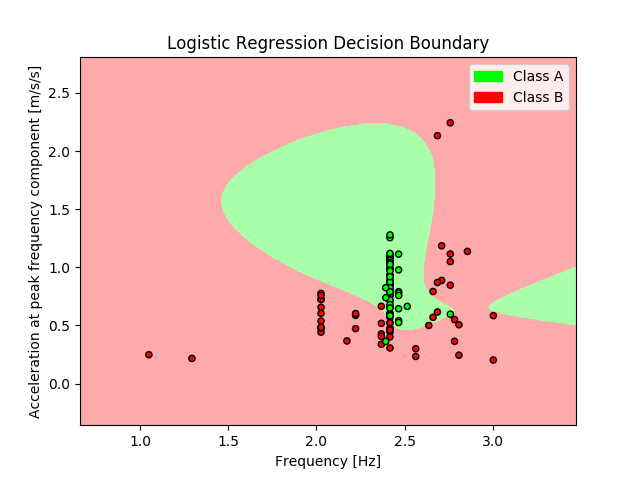
\includegraphics[scale=0.8]{logistic_regression_order10_decision_boundary_reg}
	\decoRule
	\caption{This figure shows the decision boundary from the logistic regression model using a regularization term of $\lambda=3$.  This is a 10th order model using 2 input parameters and a binary output class.  This model has an accuracy of about 86\% when using the test data set, which is higher than the 10th order model with no regularization (Figure \ref{fig:logistic_regression_order10_decision_boundary}).  This figure was created with Python.}
	\label{fig:logistic_regression_order10_decision_boundary_reg}
\end{figure}

The logistic regression function outputs the probability that the data set falls into a certain class.  This means that for most decision boundary plots, the data set is classified as Class A if the probability is greater than 50\% and the data is classified as Class B if the probability is less than 50\%.  The decision boundary can also include the probability to produce a smooth gradient plot as in Figure \ref{fig:logistic_regression_decision_boundary_smooth}.

\begin{figure}
	\centering
	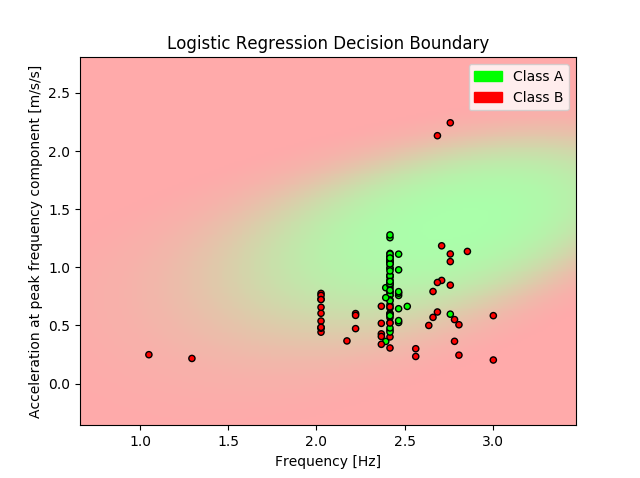
\includegraphics[scale=0.8]{logistic_regression_decision_boundary_smooth}
	\decoRule
	\caption{This figure shows the probability of the model classifying certain data sets as Class A and Class B.  This model was trained with an order of 3 and a regularization parameter of $\lambda=1$.  The background color of the plot represents the probability of the data set being classified as Class A, with solid green being about 99\% certainty and solid red being about 1\% certainty.  This figure was created with Python.}
	\label{fig:logistic_regression_decision_boundary_smooth}
\end{figure}



\subsection{Using a complete feature set}
The logistic regression models in the previous section use only 2 features from the entire data set (the features shown in Figure \ref{fig:max_balanced_freq_mag}).  This is convenient because it is easy to conceptualize and visualize.  The decision boundaries for models with 2 features can be analyzed using plots like Figure \ref{fig:logistic_regression_order10_decision_boundary_reg}.  A better version of the model would use all of the frequency spectrum data as inputs to the model.  This means that instead of using the peak amplitude and corresponding maximum frequency as model inputs, the entire FFT could be used.

Using the whole frequency spectrum means the model will have 256 features (one for the magnitude of each frequency component).  This is a lot of features to use for the KNN algorithm and will be far too slow when more training data is acquired.  The benefit of regression-based models is that the computational cost to predict the class of new data remains the same regardless of how many training examples are used to optimize the model parameters.  This means that using more data will just improve the model without slowing down the real-time calculations (it will, however, make the training time much slower).

Figure \ref{fig:logistic_regression_all_features_cost} shows a plot of the cost function value during the training process.  This is a common way of visually ensuring the model has converged to a local minimum. This produces an accuracy score of 95\% on the test data which is much higher than the scores from the 2-feature models in the previous section.

\begin{figure}
	\centering
	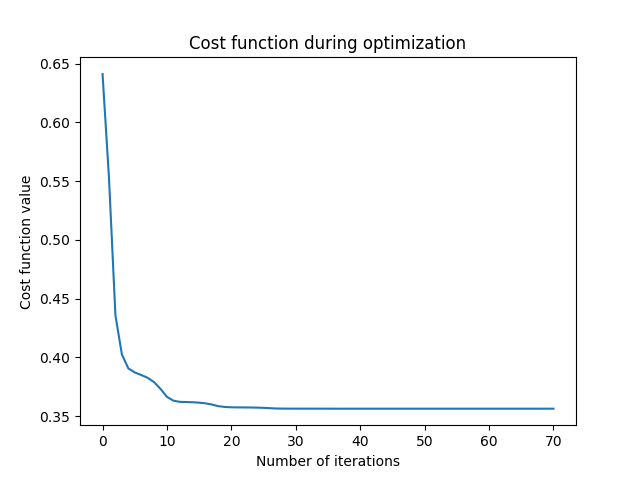
\includegraphics[scale=0.8]{logistic_regression_all_features_cost}
	\decoRule
	\caption{This figure shows the cost function value during the training process with a regularization term of $\lambda=1$.  In this model, all 256 features are used as inputs.  This figure was created with Python.}
	\label{fig:logistic_regression_all_features_cost}
\end{figure}

To better understand the results of the training process, the model parameters are plotted in Figure \ref{fig:logistic_regression_model_parameters}.  This shows each of the parameters in $\vec{\theta}$ and the corresponding frequencies they are correlated to.  To calculate the probability of the turbine being in a specific class, these parameters are multiplied with the FFT results and passed through the sigmoid function, as shown in Equation \ref{eq:logistic_regression_hypothesis}.

From inspecting Figure \ref{fig:logistic_regression_model_parameters}, it appears as though the frequency around 2.5 Hz is weighted the most, with some of the surrounding frequencies having small negative weights.  The logistic regression model essentially ``learns" that it should inspect the rotor frequency to classify the state of the turbine.    It is also interesting that frequencies +/- 0.5 Hz from the strongest component in $\vec{\theta}$ have the biggest negative weights.  From a visual inspection of the training data in one of the previous decision boundary plots (like Figure \ref{fig:logistic_regression_order10_decision_boundary_reg}), it appears as though data is likely to belong to Class A if the frequency is fairly constant around 2.5 Hz.  If the frequency diverges from this value, the training data generally falls into Class B, which is how the logistic regression model is analyzing the data and predicting the turbine state.

\begin{figure}
	\centering
	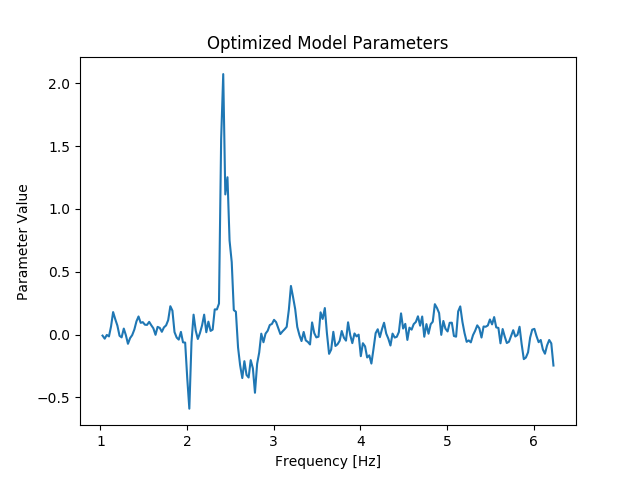
\includegraphics[scale=0.8]{logistic_regression_model_parameters}
	\decoRule
	\caption{This figure shows the optimized model parameters for the logistic regression model using all the input features.  Each parameter corresponds to a specific frequency, which means that this function gets multiplied by the FFT of each data set and used to calculate the probability that the turbine is either balanced on not balanced.  This figure was created with Python.}
	\label{fig:logistic_regression_model_parameters}
\end{figure}

\section{Neural Network}

\subsection{About the algorithm}
A neural network is an algorithm that resembles the neurons in the brain.  This is essentially a more complicated version of logistic regression, and is capable of training nonlinear models.  In some of the previous models (Such as the models in Figure \ref{fig:knn_decision_boundary_k_3} and Figure \ref{fig:logistic_regression_decision_boundary}), the DFT data was condensed down into 2 variables, which are the magnitude of the maximum frequency component and its corresponding frequency.  These variables were selected from intuition about the tower dynamics; however, there may be 2 different abstract features that better describe the system.  In order to find the 2 best features that describe the system, a neural network can be set up as shown in Figure \ref{fig:neural_network_diagram}.  This network has 3 layers, which include the input layer, hidden layer, and output layer.  The hidden layer contains 2 units, which are abstract features that can be fit to a linear model.  These 2 features should be a better indicator of the state of the turbine than the frequency and magnitude values previously used.  The (+1) units in the network represent bias units that are injected into the network to apply a constant bias to each set of parameters or features.

\begin{figure}
\centering
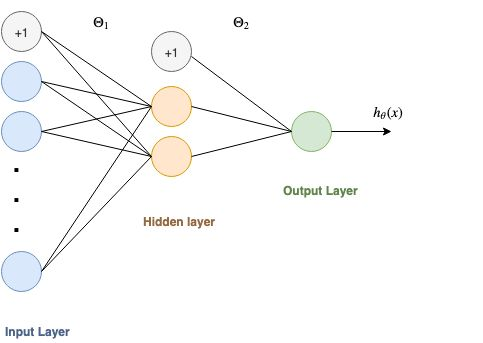
\includegraphics[scale=0.8]{neural_network_diagram}
\decoRule
\caption{This figure shows a neural network diagram for the turbine model.  The input layer contains the 256 DFT values, and the output layer contains the predicted probability that the turbine is balanced or not balanced.  The hidden layer represents some abstract features that can be used to predict the state of the turbine with a linear model.  This figure was created with Draw.io.}
\label{fig:neural_network_diagram}
\end{figure}

For each layer, the value of each unit can be calculated by multiplying the weight matrix by the previous layer units and applying the sigmoid function, $g(z)$ (Equation \ref{eq:sigmoid_function}).  For example, the values in layer 2 ($\mat{a_2}$) can be calculated using Equation \ref{eq:nn_layer_2}.
\begin{equation} \label{eq:nn_layer_2}
	\mat{a_2} = g\left(\mat{X} \cdot \mat{\Theta_1}\right)
\end{equation}

In Equation \ref{eq:nn_layer_2}, $\mat{X}$ is the input data of size $[m,n]$, where $m$ is the number of training examples, and $n$ is the number of features (256 if all the DFT values are used).  $\mat{\Theta_1}$ is the matrix of weight values that is optimized during the training process.

The hypothesis of the model in Figure \ref{fig:neural_network_diagram} is calculated using Equation \ref{eq:nn_hypothesis}.  This is the predicted probability that the turbine is balanced or unbalanced for all the training examples.
\begin{equation} \label{eq:nn_hypothesis}
	\vec{h}_{\theta} = g\left(\mat{a_2} \cdot \mat{\Theta_2} \right)
\end{equation}

The squared difference cost function of the neural network diagram is shown in Equation \ref{eq:nn_cost_function}.
\begin{equation} \label{eq:nn_cost_function}
	J(\theta) = \frac{1}{m} \sum_{i=1}^{m}{\sum_{k=1}^{K}{\left[-y_{k,i} \ln{(h_{\theta}(x_i)} - (1-y_{k,i}) \ln{(1-h_{\theta}(x_i))} \right]}}
\end{equation}

To calculate the analytic gradient of the cost function back propagation is required.  Back propagation is an algorithm is derived from calculus to determine the gradient of a neural network.  As the name suggests, this method starts from the neural network output and calculates the error of each layer, which can be related to the gradient.  First, $\delta$ for each layer is calculated as shown in Equation \ref{eq:backprop_delta_3} and Equation \ref{eq:backprop_delta_2}.  $\odot$ is the element-wise operator, which can also be represented as $\code{.*}$ in MATLAB.  It is also important to remove the term for $\delta_{2,0}$ because there is no gradient term defined for the bias unit in the second layer.
\begin{align}
	\vec{\delta}_3 &= \vec{h} - y \label{eq:backprop_delta_3}\\
	\vec{\delta}_2 &= \mat{\Theta_2}^T \cdot \vec{\delta}_3 \odot g\prime \left(\mat{X} \mat{\Theta_1}\right) \label{eq:backprop_delta_2}
\end{align}

Using $\delta$, the gradient of $\mat{\Theta_1}$ and $\mat{\Theta_2}$ can be calculated using Equation \ref{eq:backprop_theta1_grad} and Equation \ref{eq:backprop_theta2_grad}.
\begin{align}
	\frac{\partial J(\Theta)}{\partial \Theta_1} &= \frac{1}{m} \left(\vec{\delta}_2^T \cdot \vec{a}_1 \right) \label{eq:backprop_theta1_grad} \\
	\frac{\partial J(\Theta)}{\partial \Theta_2} &= \frac{1}{m} \left(\vec{\delta}_3^T \cdot \vec{a}_2 \right) \label{eq:backprop_theta2_grad}
\end{align}

The back propagation method for calculating the gradient is much faster than using a numerical method such as the finite difference approximation.  Many optimization algorithms will default to the forward finite difference gradient approximation if a gradient function is not supplied, so it is important to provide the optimization function with both the cost function and gradient function.

\subsection{Training the model}
Now that a neural network model has been set up and mathematically described, the model needs to be trained.  In other words, this means finding values for $\mat{\Theta_1}$ and $\mat{\Theta_2}$ that minimize the cost function, $J(\Theta)$.  Optimization functions generally assume the parameters are in a single vector (rather than 2 separate matrices).  $\mat{\Theta_1}$ and $\mat{\Theta_2}$ can be flattened into a single vector, and unrolled into matrices when they are used in calculations.  An example of flattening the parameters into a single vector using Python (with the numpy package) is shown below:
\begin{equation} \nonumber
	\code{nn\_params = numpy.append(Theta1.flatten(), Theta2.flatten())}
\end{equation}

To train the model, the parameters are minimized using the $\code{fmincg}$ function from the $\code{scipy.optimize}$ package.  This is a nonlinear conjugate gradient algorithm that was developed by Polak and Ribliere \cite{numerical_fmin_cg}.  Figure \ref{fig:nn_cost_function} shows the cost function during the optimization process.  \textit{It is very important that the parameters $\mat{\Theta_1}$ and $\mat{\Theta_2}$ are initialized randomly before the training process.}  If all of the values are initialized to zero, the model will not develop distinct weights for each connection.  This is a property of neural networks and is usually standard practice when training models.

\begin{figure}
\centering
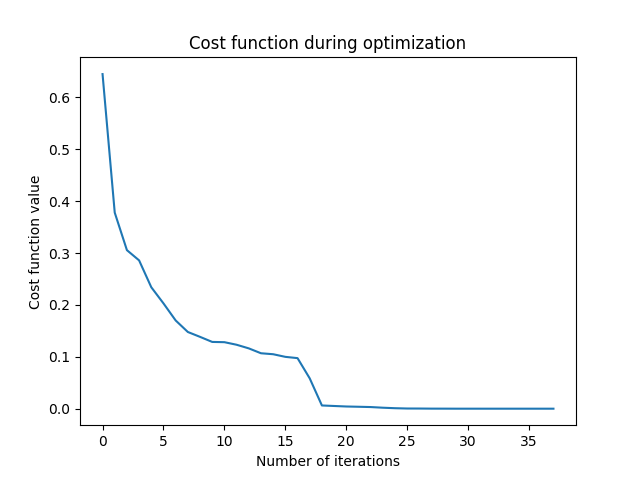
\includegraphics[scale=0.8]{nn_cost_function}
\decoRule
\caption{This figure shows the cost function of the neural network in Figure \ref{fig:neural_network_diagram} during the optimization process. This figure was created with Python.}
\label{fig:nn_cost_function}
\end{figure}

\subsection{Applying the model}
Minimizing the cost function results in optimized parameters for $\mat{\Theta_1}$ and $\mat{\Theta_2}$.  Figure \ref{fig:nn_hidden_layer_decision_boundary} shows a decision boundary plot using the hidden layer activations as input variables.  When this plot is compared to the 2-variable data in Figure \ref{fig:logistic_regression_order10_decision_boundary_reg}, the variables in Figure \ref{fig:nn_hidden_layer_decision_boundary} seem to be a much better choice of inputs.  These are abstract variables that can be fit to a linear model (notice the straight line defining the decision boundary) to describe the state of the turbine.

For clarification, the data shown in Figure \ref{fig:nn_hidden_layer_decision_boundary} are internal variables used in the neural network classification algorithm and are created from the same 256-point DFT data as the previous plots.  This model has a prediction accuracy of 85 - 95\% on the test data depending on how the variables are randomly initialized.  This variability is a result of a lack of training and test data.  For a proper neural network model more data is always better.  Unlike the nonlinear KNN algorithm, neural networks are nonlinear algorithms that have a relatively constant prediction time.  More data will not change the computational time required to calculate an output with a new test data set.

\begin{figure}
\centering
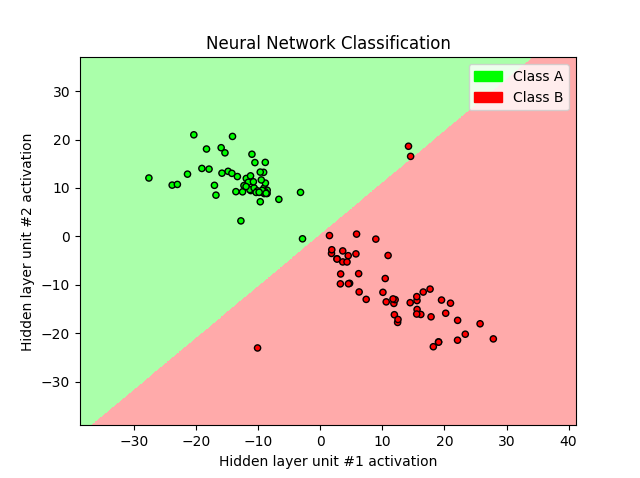
\includegraphics[scale=0.8]{nn_hidden_layer_decision_boundary}
\decoRule
\caption{This figure shows the decision boundary of the hidden layer activations of the neural network model shown in Figure \ref{fig:neural_network_diagram}.  These 2 parameters are the abstract variables that the network created to linearly classify the system. This figure was created with Python.}
\label{fig:nn_hidden_layer_decision_boundary}
\end{figure}

\subsection{Deep Learning}
A deep learning network is a neural network with multiple layer of nonlinear processing units.  The previous model was designed using the structure in Figure \ref{fig:neural_network_diagram}, which was chosen because the hidden layer only has 2 units.  This makes it easy to visualize the intermediate results of the model.  More complicated neural network models are possible, but they are harder to conceptualize and visualize.  For example, Figure \ref{fig:deep_nn_diagram} shows a version of a 6-layer neural network with 4 hidden layers.  The multiple layers in deep neural networks are abstract representations of system features.

To design a deep neural network, the Keras \cite{keras} API for TensorFlow \cite{tensorflow} is used to simplify the process.  This model has 4 hidden layers, each with 50 units per layer, which is a total of 18,551 parameters that need to be optimized when the 256 FFT values are used as inputs (shown in Table \ref{t:deep_nn_design}).  The ReLU activation function is the rectified linear unit, which is defined as $g_{relu}$ (Equation \ref{eq:relu_function}).  ReLU functions are commonly used for deep neural network hidden layer activation functions because they are cheap to compute and generally converge faster.  The sigmoid function is still required for the output layer because this needs to calculate a probability.
\begin{equation} \label{eq:relu_function}
	g_{relu}(x) = \max{(0, x)}
\end{equation}

\begin{figure}
\centering
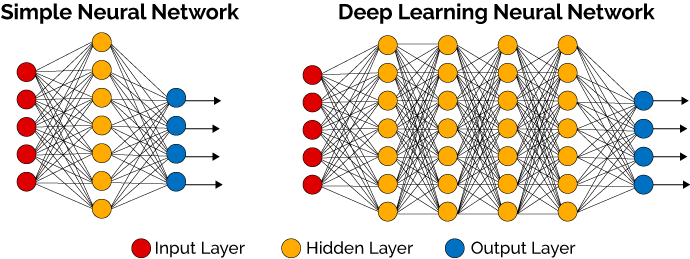
\includegraphics[scale=0.6]{deep_nn_diagram}
\decoRule
\caption{This figure shows an example of a deep learning network compared with a simple neural network (like the one in Figure \ref{fig:neural_network_diagram}) \cite{mnist_deep_learning}.}
\label{fig:deep_nn_diagram}
\end{figure}

\begin{table}[]
\centering
\caption{Deep neural network design}
\label{t:deep_nn_design}
\vspace*{0.2in}
\begin{tabular}{|c|c|c|}
\rowcolor[HTML]{EFEFEF} 
\hline
\textbf{Layer} & \textbf{Number of Units} & \textbf{Activation Function} \\ \hline
Input Layer & 256 & None \\ \hline
Hidden Layer 1 & 50 & ReLU \\ \hline
Hidden Layer 2 & 50 & ReLU \\ \hline
Hidden Layer 3 & 50 & ReLU \\ \hline
Hidden Layer 4 & 50 & ReLU \\ \hline
Output Layer & 1 & Sigmoid \\ \hline
\end{tabular}
\end{table}

This is a complex model that cannot be visualized using a decision boundary plot like the previous models.  Complex models can be prone to overfitting, which means they effectively memorize the training data and perform poorly on new test data.  Epochs, or iterations, can be manually set to limit model overfitting.  For every epoch, the training loss should be decreasing because the optimization process is taking a new step towards minimizing the loss.  If the model is actually improving, the test data loss should also be decreasing.  Once the model begins to start overfitting, the test loss will start to increase.  This shows that the model has started to memorize the training data and is not doing a good job at predicting outputs on the new (test) data.  Figure \ref{fig:python_deep_nn_loss} shows a plot of the training and test data loss over each epoch.  It can be seen that the optimum amount of epochs is about 200, because more will cause the testing loss to increase.  This can be verified in Figure \ref{fig:python_deep_nn_accuracy}, which shows the test and training data reach a maximum accuracy at about 200 epochs also.  Any more iterations (epochs) will cause the model to overfit the training data and will not improve the calculated accuracy.

When the iteration process is stopped after 200 epochs, the training data accuracy is 97\%; however, this is not expected to be a good representation of the performance of the neural network.  Test data accuracy is a much better representation because it tests the model on new data.  The test data accuracy for this model is about 91\%.

\begin{figure}
\centering
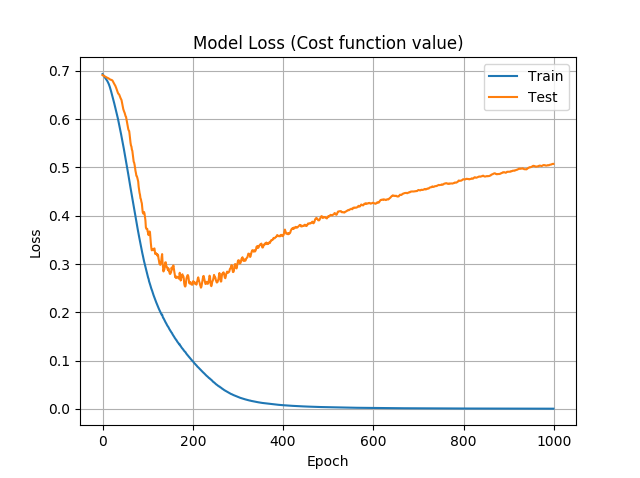
\includegraphics[scale=0.8]{python_deep_nn_loss}
\decoRule
\caption{This figure shows the loss (cost function value) for the training and test data using the model with a structure shown in Table \ref{t:deep_nn_design}.  This figure was created with Python.}
\label{fig:python_deep_nn_loss}
\end{figure}

\begin{figure}
\centering
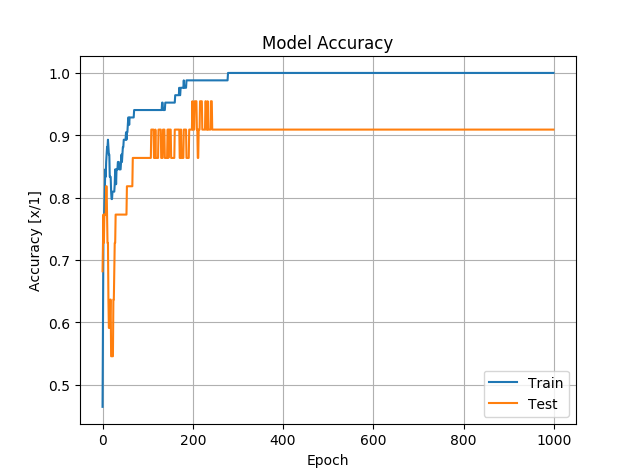
\includegraphics[scale=0.8]{python_deep_nn_accuracy}
\decoRule
\caption{This figure shows the accuracy of the training and test data using the model with a structure shown in Table \ref{t:deep_nn_design}. This figure was created with Python.}
\label{fig:python_deep_nn_accuracy}
\end{figure}




\nocite{*}
\bibliography{bibliography}

% Indents Appendix in Table of Contents
\makeatletter
\addtocontents{toc}{\let\protect\l@chapter\protect\l@section}
\makeatother

% Hack to make Appendices to appear in Table of Contents
%\addtocontents{toc}{%
%   \noindent APPENDICES
%}
%\begin{appendices}
%

%\end{appendices}

\end{document}
